\documentclass{VUMIFInfBakalaurinis}
\usepackage{algorithmicx}
\usepackage{algorithm}
\usepackage{algpseudocode}
\usepackage{amsfonts}
\usepackage{amsmath}
\usepackage{bm}
\usepackage{enumitem}
\usepackage{caption}
\usepackage{color}
\usepackage{float}
\usepackage{subcaption}
\usepackage{graphicx}
\usepackage{listings}
\usepackage{subfig}
\usepackage{wrapfig}

% Titulinio aprašas
\university{Vilniaus universitetas}
\faculty{Informatikos institutas}
\department{Programų Sistemų katedra}
\papertype{Bakalauro baigiamasis darbas}
\title{Automobilių numerių atpažinimas naudojant Tesseract LSTM rekurentinį neuroninį tinklą}
\titleineng{Car Number Plate Recognition Using Tesseract LSTM Recurrent Neural Network}
\status{4 kurso 5 grupės studentas}
\author{Emilis Ruzveltas}
\supervisor{dr. Vytautas Valaitis}
\reviewer{lekt. Tomas Smagurauskas}
\date{Vilnius \\ \the\year}

% Nustatymai
\setmainfont{Palemonas}   % Pakeisti teksto šriftą į Palemonas (turi būti įdiegtas sistemoje)
\bibliography{bibliografija} 

\definecolor{codegreen}{rgb}{0,0.6,0}
\definecolor{codegray}{rgb}{0.5,0.5,0.5}
\definecolor{codepurple}{rgb}{0.58,0,0.82}
\definecolor{backcolour}{rgb}{0.95,0.95,0.92}
 
\lstdefinestyle{mystyle}{
    backgroundcolor=\color{backcolour},   
    commentstyle=\color{codegreen},
    keywordstyle=\color{magenta},
    numberstyle=\tiny\color{codegray},
    stringstyle=\color{codepurple},
    basicstyle=\footnotesize,
    breakatwhitespace=false,         
    breaklines=true,                 
    captionpos=b,                    
    keepspaces=true,                 
    numbers=left,                    
    numbersep=5pt,                  
    showspaces=false,                
    showstringspaces=false,
    showtabs=false,                  
    tabsize=2
}
 
\lstset{style=mystyle}
\begin{document}
\maketitle
\setcounter{page}{2}
\sectionnonumnocontent{Santrauka}
% Santraukose lietuvių ir anglų kalbomis glaustai aprašomas darbo turinys: pristatoma
% nagrinėta problema ir padarytos išvados. Santraukų gale nurodomi darbo raktiniai žodžiai.
% Santraukos lietuvių ir anglų kalbomis rašomos atskiruose puslapiuose. Kiekvienos jų apimtis – ne
% daugiau kaip 0,5 puslapio. 
Darbe analizuojami dviejų tipų neuroniniai tinklai, kurių pagalba galima iš nuotraukos atpažinti automobilio numerius.

Šio darbo tikslas - sumodeliuoti dviejų tipų neuroninius tinklus bei jų pagalba atpažinti lietuviškus automobilio numerius paveikslėlyje.

Šiam tikslui atlikti buvo atskirtos dvi dalys. Pirmoje dalyje sugeneruojama, kuo panašesnių į realaus pasaulio sąlygas,
paveikslėlių, kurie panaudoti apmokyti konvoliucinė neuroninį tinklą. Vėliau tinklas apmokomas su sugeneruotais duomenimis.
Galiausiai parašoma programa, kuri randa automobilio numerio rėmelio koordinates ir išsaugo iškirptą paveikslėlį.
Antroje dalyje sugeneravus atsitiktinių automobilių numerių simbolių, buvo apmokytas Tesseract LSTM rekurentinis neuroninis
tinklas. Vėliau sukurta programa, kuri pasinaudojus gautu neuroniniu tinklu, atpažįsta simbolius esančius automobilio numeryje.
Darbe apžvelgiami būdai kaip reikia generuoti mokymo duomenis. Kaip modifikuoti paveikslėlius, norint,
kad neuroninio tinklo mokymo metu būtų pasiekti kuo geresni rezultatai.

Raktiniai žodžiai: konvoliucinis neuroninis tinklas, rekurentinis neuroninis tinklas, Tesseract, LSTM, automobilių numerių atpažinimas.
\newpage
\sectionnonumnocontent{Summary}
The paper analyzes two types of neural network, which help to recognize car number plates from image.

Aim of this work is to create a program, which can detect and recognize car number plate from image.
There are two separated parts in this paper. In the first part, there were generated images with number plates in it 
which are close to real world conditions and fed to convolutional neural network to train. Then the program was developed to 
detect number plate borders using trained neural network and save cropped image.
In the second part, there were generated random sequences of car number plates and then fed to the Tesseract LSTM recurrent 
neural network. After that, the program was developed, which recognize car number plate symbols.
This paper analyzes ways of generating different training data, how to modify images, to better train neural networks.

Key words: convolutional neural network, recurrent neural network, Tesseract, Long short-term memory, car number plate recognition.
% Santraukose lietuvių ir anglų kalbomis glaustai aprašomas darbo turinys: pristatoma
% nagrinėta problema ir padarytos išvados. Santraukų gale nurodomi darbo raktiniai žodžiai.
% Santraukos lietuvių ir anglų kalbomis rašomos atskiruose puslapiuose. Kiekvienos jų apimtis – ne
% daugiau kaip 0,5 puslapio. 

\newpage
\tableofcontents

\pagebreak
\sectionnonum{Įvadas}
% Įvade apibrėžiamas tiriamasis objektas akcentuojant neapibrėžtumą, kuris bus išspręstas
% darbe, aprašomas temos aktualumas, nurodomas darbo tikslas ir uždaviniai, kuriais bus
% įgyvendinamas tikslas, aptariamos teorinės darbo prielaidos bei metodika, apibūdinami su tema
% susiję literatūros ar kitokie šaltiniai, temos analizės tvarka, darbo atlikimo aplinkybės, pateikiama
% žinių apie naudojamus instrumentus (programas ir kt., jei darbe yra eksperimentinė dalis). Darbo
% įvadas neturi būti dėstymo santrauka. Įvado apimtis 2–4 puslapiai. 
Pagrindinis automobilių atpažinimo sistemų tikslas yra automatizuoti vaizdo stebėjimą ir
apdorojimą bei automatiškai surinkti įvairią informaciją apie transporto priemonę. Automobilių
numerių atpažinimo sistemos remiasi tuo, kad kiekviena transporto priemonė turi unikalų 
identifikacinį kodą, kuris leidžia vienareikšmiškai nustatyti transporto priemonės savininką. Techniškai
automobilių numerių atpažinimas yra paveikslėlių apdorojimo programa, naudojantis specialiu 
algoritmu išgauti rezultatus iš paveikslėlio. Automatinis paveikslėlių atpažinimas turi platų spektrą
pritaikimo sričių, tokių kaip automobilių patikra, automatinis kelių mokesčių surinkimas, išmanus
eismo reguliavimas \cite{bhushan2013license}. Didžioji dauguma automobilio numerių atpažinimo sistemų remiasi
optine ženklų atpažinimo sistema. Jų apdorojimo greitis yra pakankamai greitas, kad būtų 
efektyviai išnaudojama įvairiose srityse. Tačiau dažniausiai yra kuriamos specializuotos atpažinimo
programos skirtingiems regionams. Panaudojus neuroninius tinklus galima būtų apmokyti 
atpažinti numerius, kurių formatai yra skirtingi. Taip pat galima būtų pagreitinti procesą iškerpant
numerio rėmelį iš paveikslėlio pasinaudojus neuroniniais tinklais. Norint pagreitinti patį 
teksto atpažinimą galima naudoti rekurentinį neuroninį tinklą su LSTM savybėmis \cite{li2016reading}. Šiame
darbe naudosime kursinio darbo metu sukurtą konvoliucinį neuroninį tinklą, kuris yra skirtas 
atpažinti numerio rėmelio koordinates. Taip pat pritaikysime bei modifikuosime Tesseract LSTM
rekurentinį neuroninį tinklą, kuris sugebės atpažinti automobilio numerio simbolius \cite{smith2007overview}.

\sectionnonumnocontent{Darbo tikslas}
Sumodeliuoti dviejų tipų neuroninius tinklus bei jų pagalba atpažinti lietuviškus automobilio numerius paveikslėlyje.

\sectionnonumnocontent{Uždaviniai}
\begin{enumerate}[itemsep=0.5pt]
  \item Pasinaudojus paveikslėlių duomenų rinkiniu susigeneruoti 100.000 atsitiktinių paveikslėlių su automobilio numeriais.
  \item Apmokyti kursinio darbo metu sukurtą konvoliucinį neuroninį tinklą (rėmelio atpažinimui) pateikiant sugeneruotus paveikslėlius.
  \item Apmokyti Tesseract LSTM rekurentinį neuroninį tinklą (teksto atpažinimui) pateikiant sugeneruotus paveikslėlius.
  \item Pasinaudojus kursinio darbo metu sukurtu ir apmokytu konvoliuciniu neuroniniu tinklu atpažinti numerio rėmelį paveikslėlyje ir gauti jo koordinates.
  \item Pagal gautas koordinates, iškirpti rėmelį ir pasinaudojus Tesseract LSTM neuroniniu tinklu atpažinti numerį bei atvaizduoti gautus rezultatus pradiniame paveikslėlyje.
  \item Ištestuoti tinklą su tikrais paveikslėliais, kuriuose yra lietuviški automobilių numeriai.
\end{enumerate}

\sectionnonumnocontent{Darbo prielaidos ir metodika}
Šiais laikais, kai dominuoja naujosios technologijos, paremtos dirbtiniu intelektu, svarbu
analizuoti ir gilintis į procesus, kurie nusako kaip veikia neuroniniai tinklai. Analizuojant bei 
tobulinant dirbtinio intelekto sistemas, galima pasiekti greitesnių bei efektyvesnių rezultatų nei
naudojant tradicinius atpažinimo metodus.

Tyrimo objektas yra automobilių numerių atpažinimas. Bus tiriama kaip vyksta teksto atpažinimas pasitelkiant dirbtinius neuroninius tinklus.

Pagrindinis šio tyrimo metodas - rekurentinio LSTM dirbtinio neuroninio tinklo veikimo
analizė. Analizuojama pasitelkiant įvairius mokslinius šaltinius, straipsnius, publikacijas, knygas.
Kitoje darbo dalyje bus atliekamas eksperimentas pritaikant teoriją.

\sectionnonumnocontent{Darbo atlikimo procesas}
Pirmiausia bus gilinamasi į Tesseract LSTM neuroninio tinklo veikimo principus \cite{bhushan2013license}.
Išanalizavus, bus bandoma apmokyti neuroninį tinklą su kursinio darbo metu sugeneruotais 
paveikslėliais. Atlikus apmokymą, reikės analizuoti ir gerintį tikslumą keičiant neuroninio tinklo
specifikaciją. Galiausiai norint pasiekti dar didesnę spartą ir tikslumą, tinklas bus pritaikytas 
atpažinti lietuviškus automobilio numerius. Atlikus šį eksperimentą bus sukurta programa, kuri
naudos kursinio darbo metu sukurtą konvoliucinį neuroninį tinklą skirtą atpažinti rėmelį bei šiame
darbe sukurtą bei modifikuotą Tesseract LSTM neuroninio tinklo konfigūraciją.

\sectionnonumnocontent{Eksperimente naudojami instrumentai}
Atlikti šiam eksperimentui buvo naudojami šie pagrindiniai įrankiai:

\begin{itemize}[itemsep=0.5pt]
  \item Tesseract - skirta atpažinti numeryje esančius simbolius.
  \item Python - programavimo kalba naudota kurti programoms.
  \item TensorFlow - skirta neuroninio tinklo pagalba atpažinti numerio rėmelį nuotraukoje.
  \item OpenCV - skirta apdoroti paveikslėlius.
\end{itemize}

\pagebreak
\section{Duomenų generavimas}

\subsection{Rėmelio atpažinimui skirtų duomenų generavimas} \label{Mokymo duomenų generavimas}
Norint sukurti realiai veikiančią programą, kuri naudotų neuroninį tinklą išgauti tikėtinam rezultatui,
tinklą reikia apmokyti su dideliu kiekiu duomenų. Apmokant bet kokį neuroninį tinklą turi būti pateiktas
duomenų rinkinys su norimu gauti rezultatu. 

\subsubsection{Pirminis duomenų generavimo variantas}
Pirminis duomenų generavimo variantas, kuris buvo įgyvendintas bei sėkmingai sugeneruoti 100.000 paveikslėlių skirtų neuroninio tinklo apmokymui.

\subsubsubsection{Generavimo parametrai}
Šiam tyrimui buvo pasirinkta generuoti duomenų rinkinį, kurių kiekvienas paveikslėlis būtų 128 pikselių
pločio ir 64 pikselių ilgio. Toks pasirinktas būdas užtikrina, kad neuroninis tinklas bus pajėgus suprasti 
paveikslėlio turinį, o dydis pakankamai mažas, kad būtų galima turėti efektyviai veikiantį neuroninį tinklą.

\begin{figure}[ht!]
\begin{subfigure}{\linewidth}
  \centering
  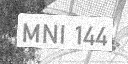
\includegraphics[width=4cm]{train_images/1_good.png}
  \captionof{figure}{Tikimasis rezultatas \textbf{MNI144 1}.}
\end{subfigure}

\begin{subfigure}{\linewidth}
  \centering
  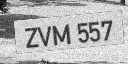
\includegraphics[width=4cm]{train_images/1_good2.png}
  \captionof{figure}{Tikimasis rezultatas \textbf{ZVM557 1}.}
\end{subfigure}

\begin{subfigure}{\linewidth}
  \centering
  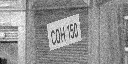
\includegraphics[width=4cm]{train_images/0_small.png}
  \captionof{figure}{Tikimasis rezultatas \textbf{COH150 0} (per mažas numeris).}
\end{subfigure}

\begin{subfigure}{\linewidth}
  \centering
  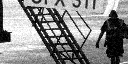
\includegraphics[width=4cm]{train_images/0_truncated.png}
  \captionof{figure}{Tikimasis rezultatas \textbf{GTK311 0} (ne pilnas numeris).}
\end{subfigure}

\begin{subfigure}{\linewidth}
  \centering
  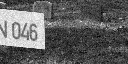
\includegraphics[width=4cm]{train_images/0_truncated2.png}
  \captionof{figure}{Tikimasis rezultatas \textbf{ABN046 0} (ne pilnas numeris).}
\end{subfigure}

\begin{subfigure}{\linewidth}
  \centering
  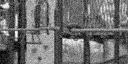
\includegraphics[width=4cm]{train_images/0_not_present.png}
  \captionof{figure}{Tikimasis rezultatas \textbf{KLF155 0} (nėra numerio).}
\end{subfigure}
\captionof{figure}{Sugeneruotų paveikslėlių pavyzdžiai}
\label{img_ex}
\end{figure}
Pirmoji paveikslėlio rezultato dalis nurodo, koks yra teisingas numeris. Antroji - numerio rėmelio egzistavimas paveikslėlyje.
Jei reikšmė 1 - numeris yra tinkamas nuskaitymui, 0 - neatitinka kriterijų (\ref{img_ex} pav.). 

Kriterijai, kurie nusako ar numerio rėmelis yra tinkamas apdorojimui:

\begin{itemize}[itemsep=0.5pt]
  \item Visas rėmelio plotas yra paveikslėlyje.
  \item Rėmelio plotis yra mažesnis nei 80\% paveikslėlio pločio.
  \item Rėmėlio aukštis yra mažesnis nei 87,5\% paveikslėlio aukščio.
  \item Rėmelio plotis yra didesnis nei 60\% paveikslėlio pločio.
  \item Rėmėlio aukštis yra didesnis nei 60\% paveikslėlio aukščio.
\end{itemize}

Su tokiais parametrais galima naudoti judantį 128x64 pikselių langelį, kuris judėtų po 8 pikselius ir kas kartą padidintų rėmelį
\begin{math}
  \sqrt{2}
\end{math}
kartų. Tokiu būdu užtikrinama, kad nebus praleista nei viena paveikslėlio vieta, o taip pat pakankamai efektyviai ir greitai pereinamas
visas paveikslėlis.

\begin{minipage}{\linewidth}
  \centering
  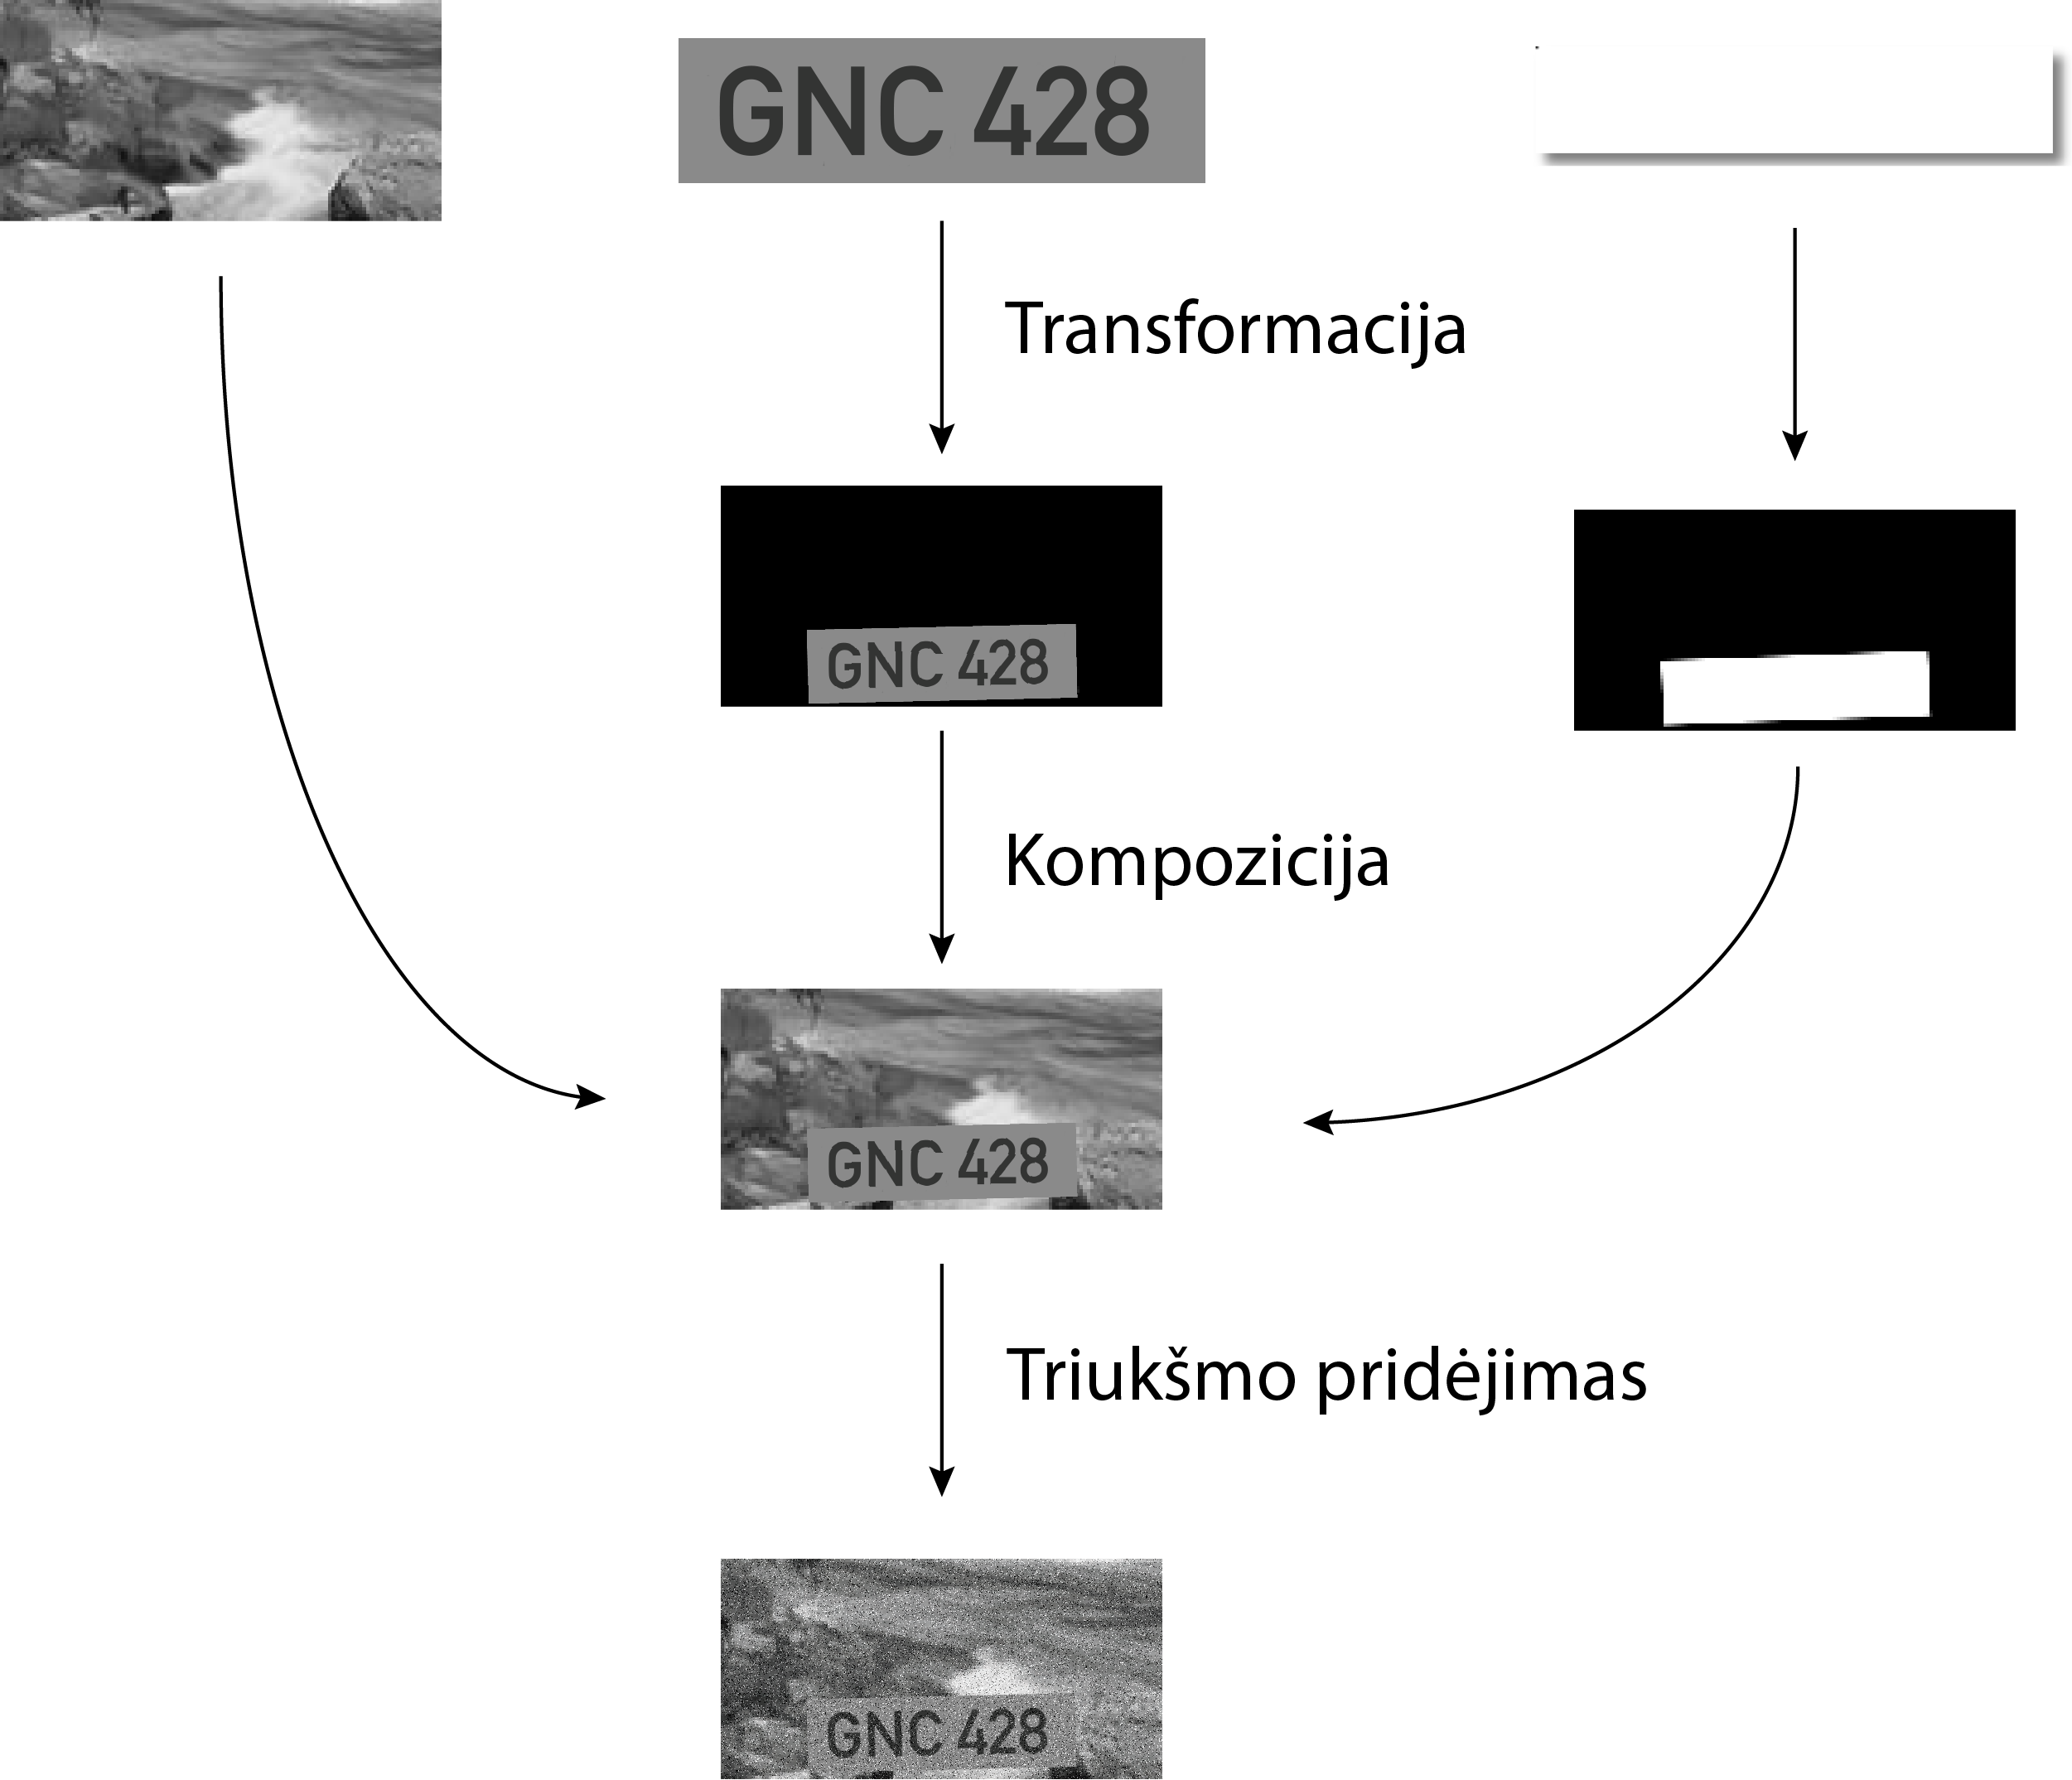
\includegraphics[width=8cm]{train_images/generating.png}
  \captionof{figure}{Paveikslėlių generavimo schema}
  \label{gen_img}
\end{minipage}

\subsubsubsection{Numerio generavimas}
Numeris ir rėmelio spalva generuojama atsitiktinai, tačiau tekstas turi būti tamsesnis negu rėmelis. Tokiu būdu bandoma atkurti realaus pasaulio apšvietimo variacijas.
Numeris generuojamas pagal Lietuvos Respublikos Valstybinių numerių formatą, kuris yra - 3 lotyniško alfabeto
raidės (išskyrus lietuvių kalboje nenaudojamas raides) ir 3 arabiški skaičiai. Generuojant numerį, 
atsitiktine tvarka parenkamos trys raidės iš 23 raidžių žodyno \textit{ABCDEFGHIJKLMNOPRSTUVYZ} bei 3 skaičiai 
iš skaičių žodyno \textit{0123456789}. Maksimalus galimas unikalių numerių skaičius siekia:
\begin{equation}
  23^3 * 10^3 = 12.167.000.
\end{equation}

\subsubsubsection{Transformacija}

Norint, kad tinklas efektyviai mokytųsi ir atpažintų paveikslėlius realaus pasaulio sąlygomis, generuojant duomenų
rinkinį buvo pritaikyta remėlio transformacija. Tai atlikti buvo pasitelktas metodas generuoti atsitiktines
reikšmes X, Y, Z ašims ir pritaikyti Oilerio kampų metodą\cite{slabaugh1999computing}. 
Reikšmių rėžiai pasirinkti tokie, kuriuos labiausiai tikėtina sutikti realiame pasaulyje.
Kaip atrodo transformacija galima matyti \ref{gen_img} paveikslėlyje.
Ašių atsitiktinių reikšmių rėžiai:
\begin{equation}
  -0.3 \leq X \leq 0.3,
\end{equation}
\begin{equation}
  -0.2 \leq Y \leq 0.2,
\end{equation}
\begin{equation}
  -1.2 \leq Z \leq 1.2.
\end{equation}

Transformacijos vykdomos 3 etapais (programinis kodas matomas \ref{euler_img} pav.):
\begin{enumerate}[itemsep=0.5pt]
  \item Sukama aplink Y ašį:
  \begin{itemize}[itemsep=0.5pt]
    \item Apskaičiuojamos cos(Y) ir sin(y) reikšmės,
    \item Sudaroma 3x3 matrica su reikšmėmis,
    \begin{equation}
      \begin{bmatrix}
        c & 0 & s \\
        0 & 1 & 0 \\
        -s & 0 & c
      \end{bmatrix}
      .
    \end{equation}
  \end{itemize}
  \item Sukama aplink X ašį
  \begin{itemize}[itemsep=0.5pt]
    \item Apskaičiuojamos cos(X) ir sin(X) reikšmės,
    \item Sudaroma 3x3 matrica su reikšmėmis,
    \begin{equation}
      \begin{bmatrix}
        1 & 0 & 0 \\
        0 & c & -s \\
        0 & s & c
      \end{bmatrix}
      .
    \end{equation}
    \item Sudauginama su praeitame žingsnyje gauta matrica
  \end{itemize}
  \item Sukama aplink Z ašį
  \begin{itemize}[itemsep=0.5pt]
    \item Apskaičiuojamos cos(Z) ir sin(Z) reikšmės,
    \item Sudaroma 3x3 matrica su reikšmėmis, 
    \begin{equation}
      \begin{bmatrix}
        c & 0 & s \\
        0 & 1 & 0 \\
        -s & 0 & c
      \end{bmatrix}
      ,
    \end{equation}
    \item Sudauginama su praeitame žingsnyje gauta matrica.
  \end{itemize}
\end{enumerate}

\begin{minipage}{\linewidth}
  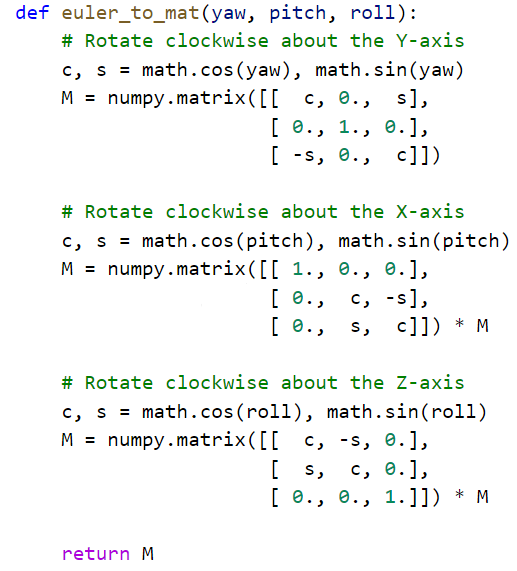
\includegraphics[width=8cm]{euler.png}
  \captionof{figure}{Oilerio kampų metodo kodas}
  \label{euler_img}
\end{minipage}

\subsubsubsection{Kompozicija}
Turėti realų foną svarbu, kadangi tinklas turi išmokti surasti rėmelio kampus „nesukčiaudamas“. 
Naudojant juodą foną, tinklas gali daryti prielaidą, kad remėlis yra ten, kur nėra juodos spalvos, o tai būtų netikslu realiame pasaulyje.
Transformuotas automobilio numerio rėmelis sukomponuojamas su atsitiktiniu paveikslėliu atsitiktinėje vietoje.
Atsitiktinių paveikslėlių šaltiniu naudojamas daugiau nei 100.000 paveikslėlių duomenų rinkinys \cite{xiao2010sun}.
Labai svarbu didelis kiekis paveikslėlių, taip sumažinant riziką, kad neuroninis tinklas atsimins kiekvieną paveikslėlį.
Kaip atrodo kompozicija galima matyti \ref{gen_img} paveikslėlyje.
\begin{equation}
  A = 0.6,
\end{equation}
\begin{equation}
  B = 0.875,
\end{equation}
\begin{equation}
  C = 1.5.
\end{equation}
kur:
\begin{itemize}[itemsep=0.5pt]
  \item A - minimalus numerio rėmelio plotis,
  \item B - maksimalus numerio rėmelio aukštis,
  \item C - dydžio variacijos koeficientas.
\end{itemize}
\begin{equation}
  min = (A + B) * 0.5 - (B - A) * 0.5 * C,
\end{equation}
\begin{equation}
  min = ((0.6 + 0.875) * 0.5) - ((0.875 - 0.6) * 0.5 * 1.5),
\end{equation}
\begin{equation}
  min = (1.475 * 0.5) - (0.275 * 0.5 * 1.5),
\end{equation}
\begin{equation}
  min = 0.7375 - 0.20625,
\end{equation}
\begin{equation}
  \textbf{min = 0.53125},
\end{equation}
\begin{equation}
  max = (A + B) * 0.5 + (B - A) * 0.5 * C,
\end{equation}
\begin{equation}
  max = ((0.6 + 0.875) * 0.5) + ((0.875 - 0.6) * 0.5 * 1.5),
\end{equation}
\begin{equation}
  max = (1.475 * 0.5) + (0.275 * 0.5 * 1.5),
\end{equation}
\begin{equation}
  max = 0.7375 + 0.20625,
\end{equation}
\begin{equation}
  \textbf{max = 0.94375},
\end{equation}
\begin{equation}
  x = R[min, max],
\end{equation}
\begin{equation}
  p = 1, \text{kai } x \in [A, B],
\end{equation}
\begin{equation}
  p = 0, \text{kai } x \in [A, B].
\end{equation}
kur:
\begin{itemize}[itemsep=0.5pt]
  \item min - minimalus generuojamas dydžio koeficientas,
  \item max - maksimalus generuojamas dydžio koeficientas,
  \item R - atsitiktinio skaičiaus generavimo funkcija tarp dviejų reikšmių,
  \item x - numerio rėmelio dydžio koeficientas lyginant su pradiniu dydžiu,
  \item p - jei 1 - rėmelis tinkamai egzistuoja paveikslėlyje, 0 - rėmelis neegzistuoja arba yra netinkamas.
\end{itemize}

Atsitiktinių reikšmių rėžis, kuris nusako kurioje vietoje turėtų atsidurti rėmelis.

\subsubsubsection{Triukšmo pridėjimas}
Triukšmas paveikslėlyje reikalingas, kadangi realiame pasaulyje pasitaiko, kad kameros sensorius generuoja triukšmus, o taip pat,
kad neuroninis tinklas nepersimokytų ir neskirstytų paveikslėlių pagal vieną konkrečią spalvą ar būtų priklausomas nuo „aštrių“ kampų.
Triukšmas paveikslėliui pridedamas pritaikant Gauso normalųjį skirstinį su reikšme 0.05.
Kaip atrodo triukšmo pridėjimas galima matyti \ref{gen_img} paveikslėlyje.

\subsection{Numerio atpažinimui skirtų duomenų generavimas}
Norint sėkmingai apmokyti neuroninį tinklą, reikia daug pradinių mokymo duomenų. Šiam tikslui pasiekti nuspręsta duomenis susigeneruoti, kadangi tiek daug lietuviškų numerių
tikrų nuotraukų nėra įmanoma gauti. 

\subsubsection{Idėja}
Norint kuo efektyviau apmokyti LSTM rekurentinį neuroninį tinklą, reikia sugeneruoti tokio pačio šrifto atsitiktinius numerius, kurie kuo panašiau atkurtų realią situaciją. 
Idėja buvo susirinkti visas galimas raides ir skaičius iš realių automobilių nuotraukų. Atrinktus simbolius išsikirpti bei sugeneruoti atsitiktinius raidžių ir skaičių kratinius.

\subsubsection{Simbolių rinkimas}
Realių automobilių numerių nuotraukų paieška buvo vykdoma http://autoplius.lt puslapyje.
Norint iškirpti kokybiškas raides bei skaičius reikia aukštos kokybės nuotraukų. 
Atrinkus tinkamas nuotraukas, buvo iškirptos visos galimos raidės ir skaičiai (\ref{symbols} pav.).
Kai kuriems simboliams reikėjo pritaikyti transformacijas, kad jų orientacija būtų horizontaliai tiesi.

\begin{minipage}{\linewidth}
  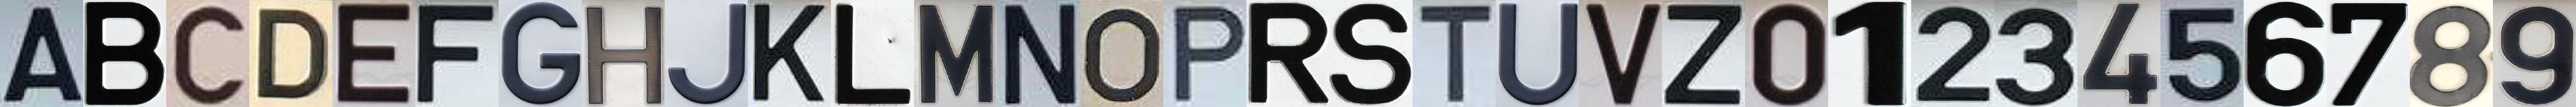
\includegraphics[width=8cm]{symbols.jpg}
  \captionof{figure}{Atrinktos raidės ir skaičiai}
  \label{symbols}
\end{minipage}

\subsubsection{Generavimo algoritmas}
Generuoti atsitiktiniams automobilio numeriams parašyta Python programėlė (žiūrėti priede \ref{generating}).
Veikimo eiga:
\begin{itemize}[itemsep=0.5pt]
  \item Masyve \textit{letters} saugomi paveikslėliai atitinkantys raides.
  \item Masyve \textit{numbers} saugomi paveikslėliai atitinkantys skaičius.
  \item Sukamas ciklas \textit{N} kartų.
  \item Kiekvieno iteracijos metu atsitiktiniu būdu atrenkamos trys raidės ir trys skaičiai iš atitinkamo masyvo.
  \item Sukuriamas naujas masyvas, kuriame iš eilės sudedami atrinkti paveikslėliai.
  \item Surandamas mažiausias paveikslėlis iš atrinktų, ir pagal jo dydį sumažinamas likusių paveikslėlių aukštis proporcingai.
  \item Sujungiamas vienas paveikslėlis iš atrinktų simbolių.
  \item Paveikslėlis išsaugomas \textit{xxxyyy.tif} formatu, kur x - raidė, y - skaičius.
  \item Šalia išsaugomas tekstinė rinkmena \textit{xxxyyy.gt.txt}, kur x - raidė, y - skaičius, kurio viduje yra XXXYYY formatu išsaugotas sugeneruotas numeris.
\end{itemize}


\pagebreak
\section{Neuroninių tinklų architektūra}
Šiame skyriuje aprašyti dviejų skirtingų neuroninių tinklų architektūriniai sprendimai.
Numerio rėmelio atpažinimui naudojamas konvoliucinis neuroninis tinklas bei 
numeryje esančių simbolių atpažinimui naudojamas rekurentinis neuroninis tinklas.

\subsection{Numerio rėmelio atpažinimui skirtas neuroninis tinklas}
Numerio rėmelio atpažinimui panaudotas konvoliucinis neuroninis tinklas.

\subsubsection{Modelis}
Neuroninis tinklas kurtas su Tensorflow bibliotekomis.
Kuriant dirbtinį konvoliucinį neuroninį tinklą buvo pasirinkta architektūra pavaizuota \ref{fig:test} pav.
Iš viso yra 3 konvoliuciniai lygiai, kurių dydžiai yra 48, 64 ir 128\cite{goodfellow2013multi}.
Visų jų langelio dydis yra vienodas - 5x5.
Taip pat yra 3 max pool'ingo lygmenys, kurių pirmo ir trečio langelio dydis yra 2x2, o antro - 1x2.
Tada neuroninis tinklas turi du pilnai sujungtus lygius, kurių pirmojo dydis - 2048, o antrojo (klasifikatoriaus) - 1.
Po pirmojo konvoliucinio lygio pritaikyta neuronų atmetimo operacija, norint nepermokyti tinklo pirminėje stadijoje.
Po trečiojo konvoliucinio lygio taip pat pritaikyta neuronų atmetimo operacija, norint padidinti neuroninio tinklo tikslumą, 
kadangi pastebėta, kad ignoruojant 50\% neuronų, tinklas turi didesnį atpažinimo tikslumą\cite{stark2015captcha}.
Kiekvieno mokymo ciklo metu imties dydis yra 50. Galutinis tinklo išvedamas rezultatas yra:
\begin{equation}
  0 \leq x \leq 1, x \in N.
\end{equation}

Neuroninį tinklą sudaro:

\begin{itemize}[itemsep=0.5pt]
  \item 3 konvoliuciniai lygiai:
    \begin{enumerate}[itemsep=0.5pt]
      \item Konvoliucinis lygis - 48 filtrų, langelio dydis 5x5, įeinančio paveikslėlio dimensijos 128x64x3, išeinančio paveikslėlio dimensijos 128x64x48.
      \item Konvoliucinis lygis - 64 filtrų, langelio dydis 5x5, įeinančio paveikslėlio dimensijos 64x32x48, išeinančio paveikslėlio dimensijos 64x32x64.
      \item Konvoliucinis lygis - 128 filtrų, langelio dydis 5x5, įeinančio paveikslėlio dimensijos 64x16x64, išeinančio paveikslėlio dimensijos 64x16x128.
    \end{enumerate}
  \item 3 max pool'ingo lygiai:
    \begin{enumerate}[itemsep=0.5pt]
      \item Max pool'ingo lygis - langelio dydis 2x2, įeinančio paveikslėlio dimensijos 128x64x48, išeinančio paveikslėlio dimensijos 64x32x48.
      \item Max pool'ingo lygis - langelio dydis 1x2, įeinančio paveikslėlio dimensijos 64x32x64, išeinančio paveikslėlio dimensijos 64x16x64.
      \item Max pool'ingo lygis - langelio dydis 2x2, įeinančio paveikslėlio dimensijos 64x16x128, išeinančio paveikslėlio dimensijos 32x8x128.
    \end{enumerate}
  \item 2 pilnai sujungti lygiai:
    \begin{enumerate}[itemsep=0.5pt]
      \item Pilnai sujungtas lygis - įeinančio paveikslėlio dimensijos 32x8x128, išeinančių signalų kiekis - 2048.
      \item Pilnai sujungtas lygis - įeinančių signalų kiekis - 2048, išeinančių signalų kiekis - 1.
    \end{enumerate}
\end{itemize}


\begin{minipage}{\linewidth}
  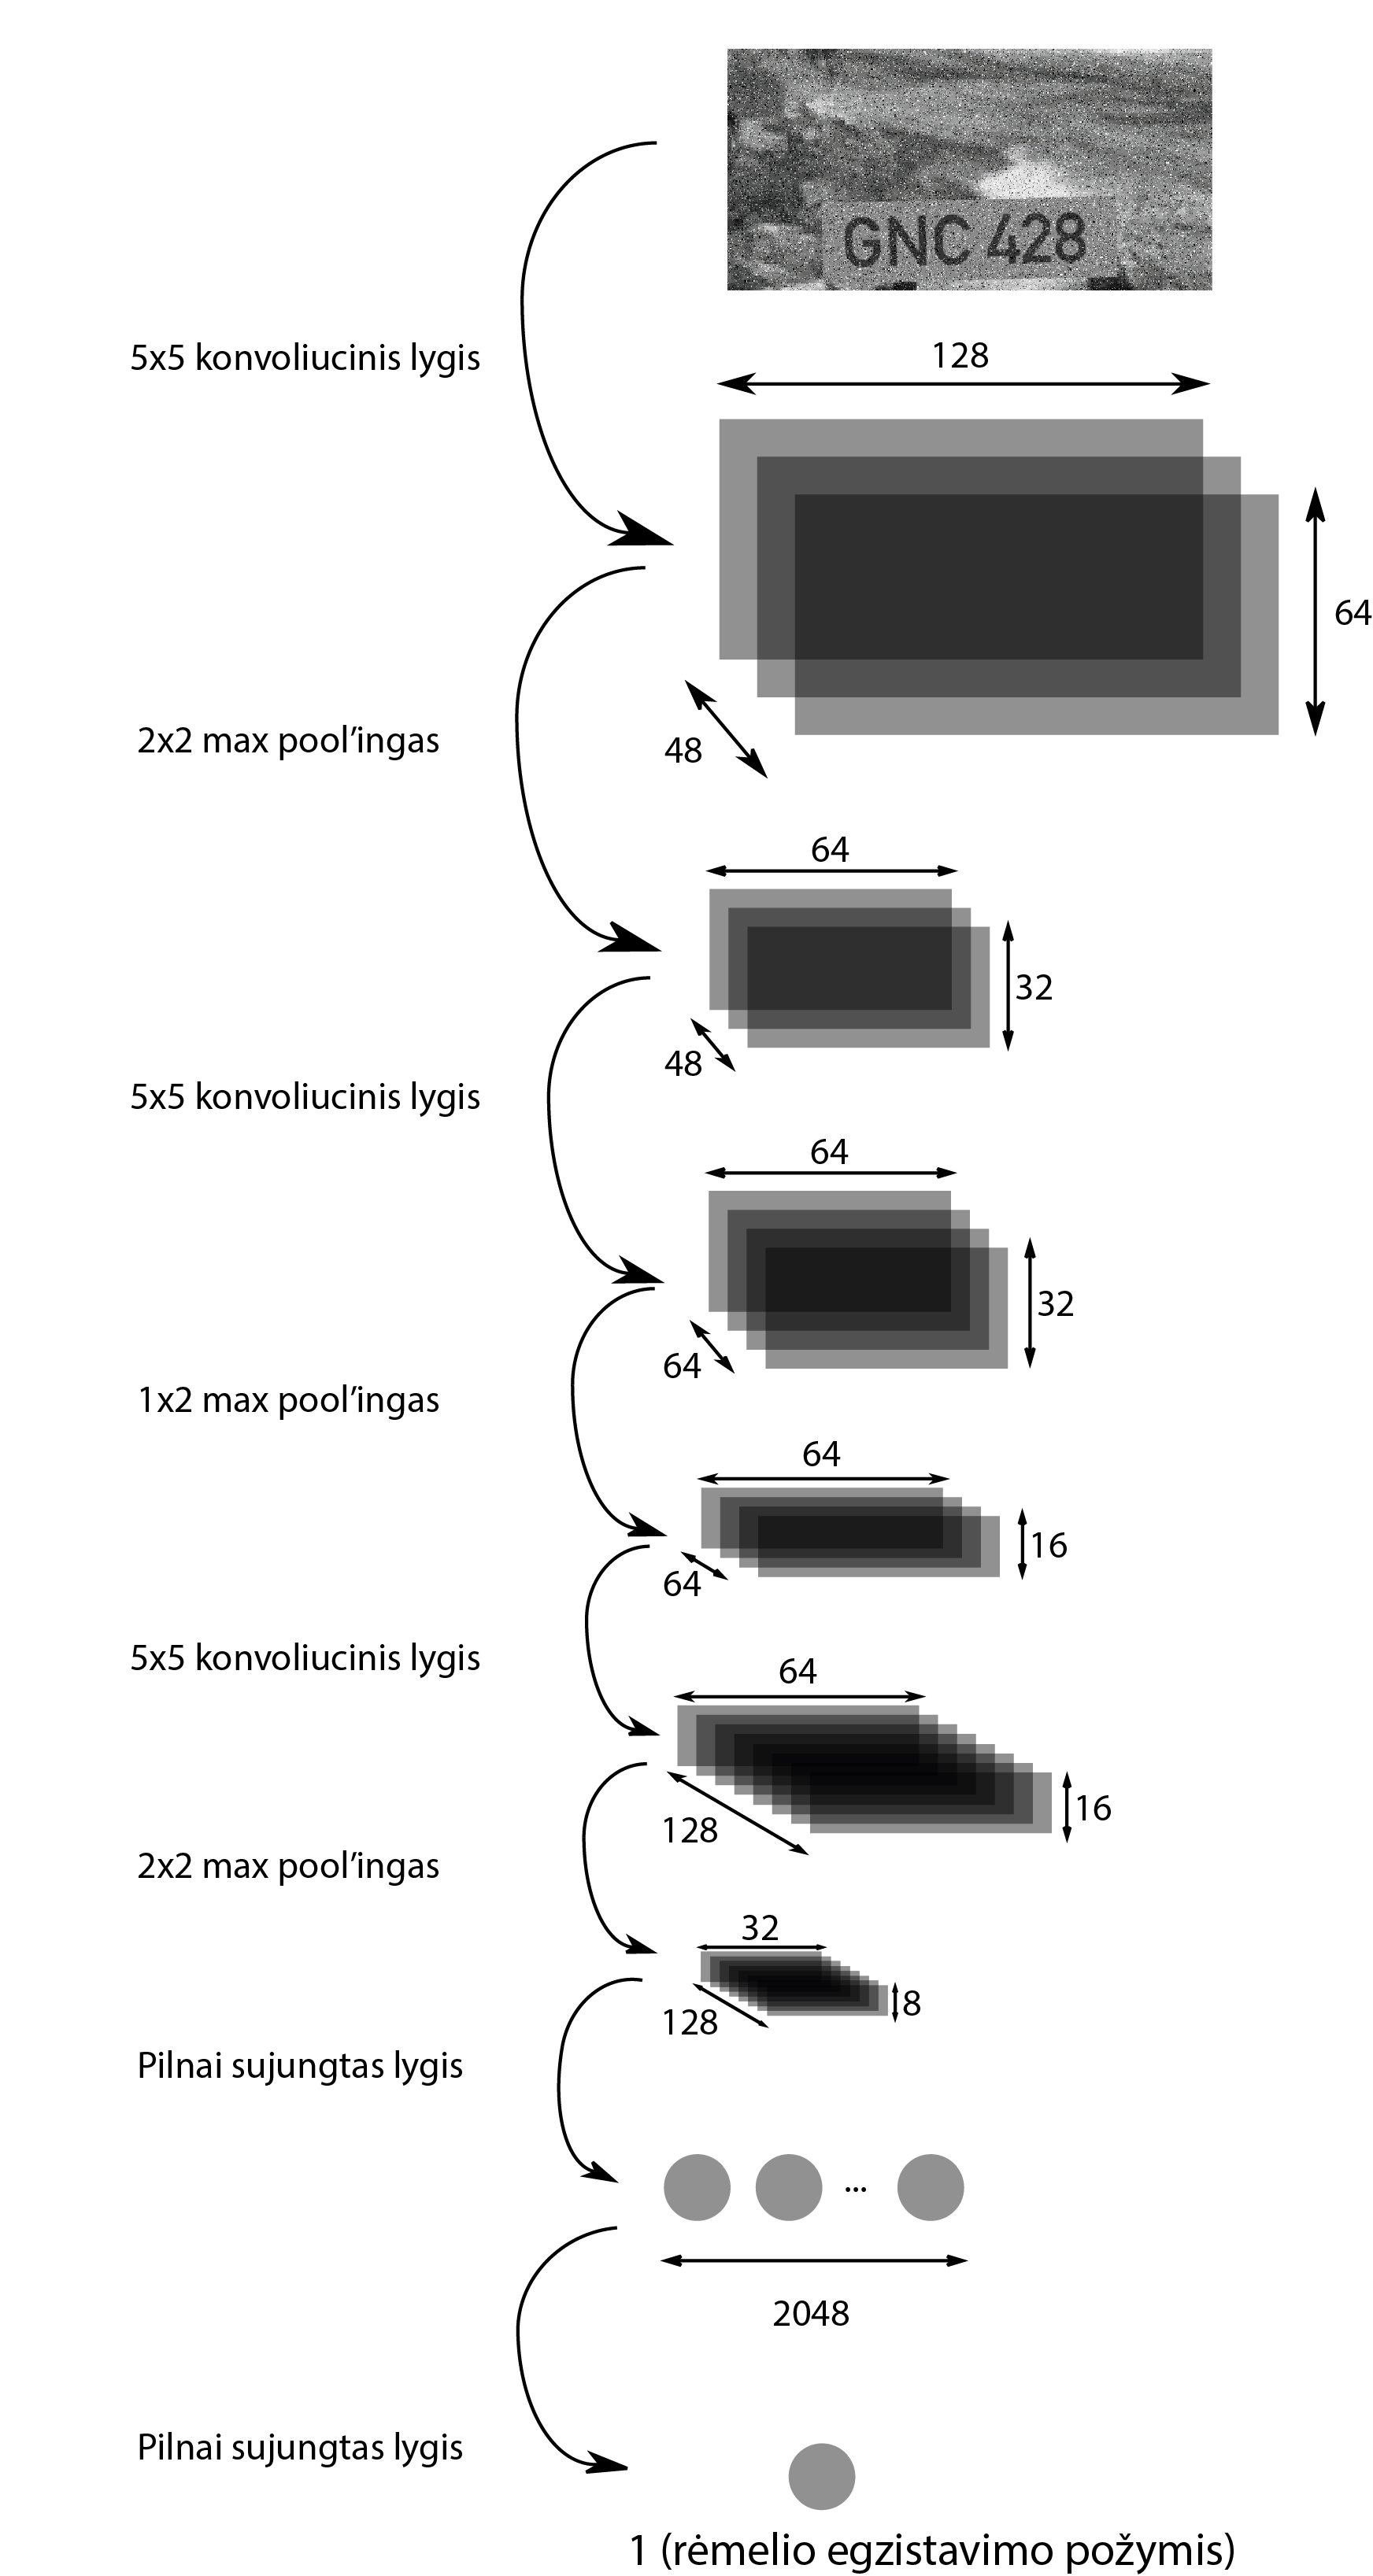
\includegraphics[width=10cm]{topology.png}
  \captionof{figure}{Neuroninio tinklo architektūra}
  \label{fig:test}
\end{minipage}

\subsection{Numerio simbolių atpažinimui skirtas neuroninis tinklas}
Tesseract programa nuo 4.00 versijos integravo naują neuroninio tinklo pagrindu veikiančią teksto eilučių atpažinimo posistemę.
Pirminis idėjos šaltinis kilo iš \textit{OCRopus} sistemos, kuri panaudodama Python programavimo kalbą įgyvendino LSTM veikimą.
Tačiau tai buvo visiškai perdaryta panaudojus C++ kalbos ypatumus.
Neuroninio tinklo sistema Tesseract programoje egzistuoja jau nuo \textit{TensorFlow} atsiradimo ir taip pat su ja yra suderinama,
kadangi naudojama tos pačios sintaksės neuroninio tinklo modelio aprašymo kalbą (VGSL)\footnote{https://github.com/tesseract-ocr/tesseract/wiki/VGSLSpecs}.

Pagrindinė VGSL idėja yra, kad nebūtina išmokti daug naujų dalykų, kad būtų įmanoma sukurti ir apkomyti neuroninį tinklą.
Nereikia mokytis \textit{Python} programavimo kalbos, \textit{TensorFlow} bibliotekos ar net rašyti C++ programinio kodo.
Užtenka įvaldyti VGSL kalbos sintaksines ypatybes, kad būtų įmanoma taisyklingai sudaryti neuroninį tinklą.

\subsubsection{Bendrai apie LSTM}
LSTM yra rekurentinio neuroninio tinklo architektūra naudojama gilaus mokymosi srityse.
Skirtingai nuo standartinių „feedforward“ neuroninių tinklų, LSTM turi grįžtamuosius ryšius, kurie tai padaro „universaliu kompiuteriu“ 
(t.y. galima skaičiuoti viską, ką gali Turingo mašina). LSTM neuroniniai tinklai gali apdoroti ne tik statinius objektus (paveikslėlius), 
bet ir informacijos sekas (garso įrašas ar video įrašas). LSTM dažniausiai naudojama ranka rašyto teksto ar garso atpažinimui \cite{hochreiter1997long}.

LSTM tinklo paslėptame rekurentiniame lygyje yra specialūs vienetai - atminties blokai (\ref{memory_block} pav.).
Atminties blokuose yra atminties ląstelių saugančių laikiną tinklo būseną pridedant dar specialius 
dauginamuosius vienetus, taip vadinamus vartus, kurie kontroliuoja informacijos srauto tėkmę.
Kiekvienas atminties blokas originalioje architektūroje yra sudarytas iš įvesties ir išvesties vartų.
Įvesties vartai kontroliuoja įvesties aktyvacijų informacijos tėkmę į atminties ląstelę.
Išvesties vartai kontroliuoja ląstelių aktyvacijos išvesties informacijos tėkmę atgal į tinklą.
Vėliau į atminties bloką pridedami atminties praradimo vartai. 
Tai sprendžia vieną iš LSTM modelio silpnybių, kai įvestis nėra suskirstyta į atskiras sekas ir apdorojimas niekad nesibaigia.
Atminties praradimo vartai keičia vidinę ląstelės būseną prieš patalpinant ją į ląstelę per rekurentinį ryšį su pačia savim,
tuo pačiu įgalinant pamiršti ar ištrinti ląstelės atmintį.
LSTM tinklas skaičiuoja sąryšius nuo įvesties sekos
\begin{equation}
  x = (x1, ..., xT) 
\end{equation}
iki išvesties sekos
\begin{equation}
  y = (y1, ..., yT)
\end{equation}
atlikdamas tinklo vienetų aktyvacijų funkcijas pagal žemiau nurodytas formules iš eilės nuo t = 1 iki T:
\begin{equation}
  i_t = \sigma(W_{ix}x_t + W_{im}m_{t−1} + W_{ic}c_{t−1} + b_i)
\end{equation}
\begin{equation}
  f_t = \sigma(W_{fx}x_t + W_{fm}m_{t−1} + W_{fc}c_{t−1} + b_f)
\end{equation}
\begin{equation}
  c_t = f_t \odot c_{t−1} + i_t\odot g(W_{cx}x_t + W_{cm}m_{t−1} + b_c)
\end{equation}
\begin{equation}
  o_t = \sigma(W_{ox}x_t + W_{om}m_{t−1} + W_{oc}c_t + b_o)
\end{equation}
\begin{equation}
  m_t = o_t \odot h(c_t)
\end{equation}
\begin{equation}
  y_t = \phi(W_{ym}m_t + b_y)
\end{equation}
kur \textit{W} apibrėžia svorių matricas (pvz.: \(W_{ix}\) yra svorių matrica nuo įvesties vartų iki pačios įvesties), 
\(W_{ic}\), \(W_{fc}\), \(W_{oc}\) yra įstrižos svorių matricos skirtos skylučių jungtims
\footnote{Skylutės jungtis (angl. peephole connection) - LSTM tinklo ypatybė, kai vartai priklausoma ne tik nuo buvusios paslėptos būsenos, bet ir nuo buvusios vidinės būsenos)},
\textit{b} apibūdina išvesties vektorius, kurie neturi jokios įvesties,
\(\sigma\) yra logistinė sigmoidinė funkcija, \textit{i}, \textit{f}, \textit{o}, \textit{c} yra atitinkamai
įvesties vartai, atminties praradimo vartai, išvesties vartai ir ląstelės aktyvacijos vektoriai, kurių visų dydis yra toks pat 
kaip ir ląstelės išvesties aktyvacijos vektoriaus \textit{m}, \(\odot\) yra vektorių elementas, \textit{g} ir \textit{h} yra ląstelės
įvestis ir ląstelės išvesties aktyvacijos funkcijos, \textit{tanh} ir \(\phi\) yra tinklo išvesties aktyvacijos funkcija - \textit{Softmax} \cite{sak2014long}.

\begin{minipage}{\linewidth}
  \centering
  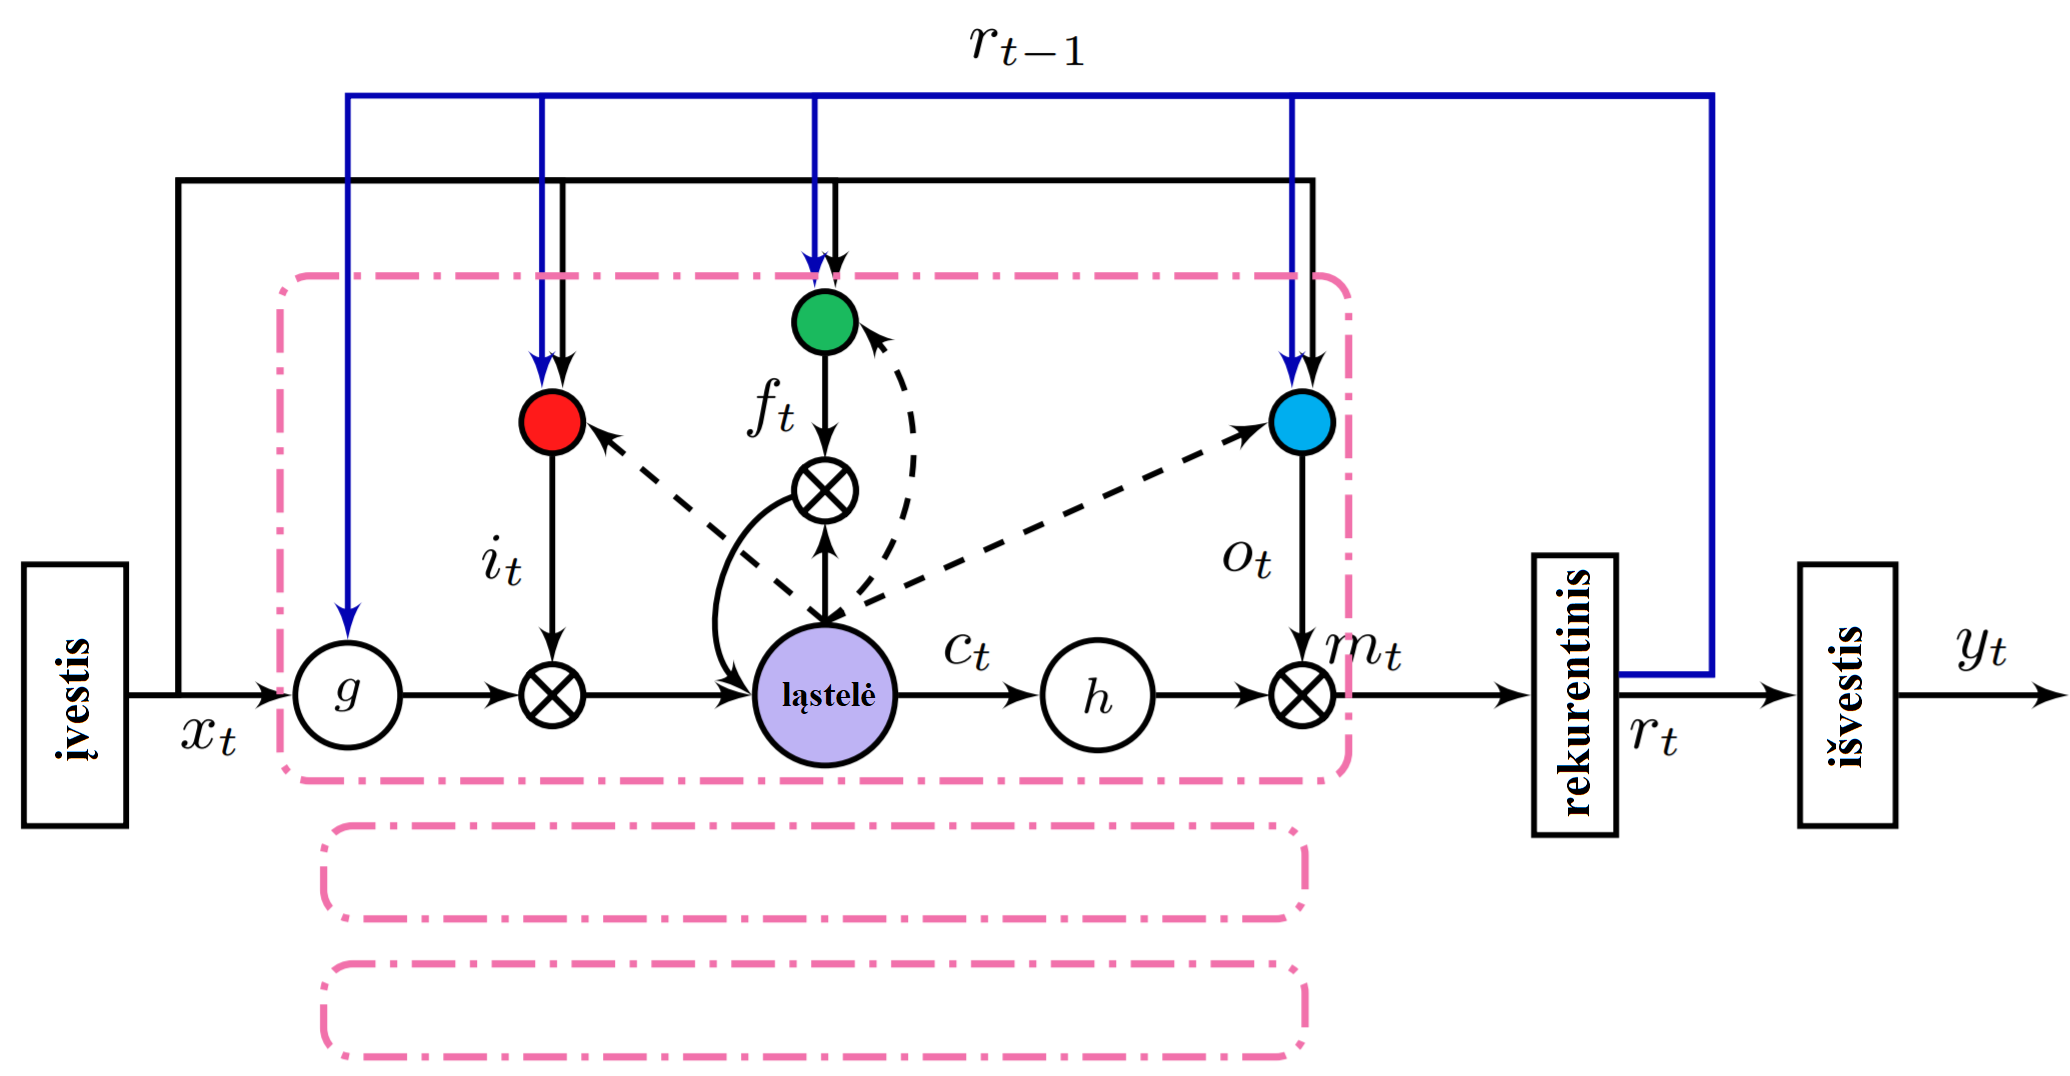
\includegraphics[width=12cm]{memory_block.png}
  \captionof{figure}{LSTM atminties blokai}
  \label{memory_block}
\end{minipage}

\subsubsubsection{Rekurentinis neuroninis tinklas}
Rekurentinis neuroninis tinklas - skirtingai nuo grįžtamuoju ryšiu grįstų neuroninių tinklų, yra rekursinio 
dirbtinio neuroninio tinklo variantas, kuriame ryšiai tarp neuronų sudaro apskritą ratą. Tai reiškia,
kad išvedimo rezultatas priklauso ne tik nuo dabartinių įvesčių, bet ir nuo ankstesnio etapo neuronų būklės. 
Šis metodas leidžia vartotojams išspręsti problemas, susijusias su balso ar kalbos atpažinimu.
Atlikti tyrimai rodo, kad įmanoma sukurti rekurentinį neuroninį tinklą, kuris gali generuoti naujus sakinius ir dokumentų santraukas.

\subsubsection{Integracija su Tesseract}
Integruota neuroninio tinklo posistemė gali būti panaudojama kaip papildinys esamai analizės sistemai atpažįstant tekstą dideliame dokumente arba
gali būti naudojama kartu su išoriniu teksto detektoriumi, kad atpažintų tekstą iš vienos teksto eilutės atvaizdo.

Nuo 4.00 versijos neuronio tinklo pagrindu veikiantis atpažinimo būdas Tesseract programoje yra numatytasis. 

\subsubsection{Sisteminiai reikalavimai}
Nauja programos versija naudoja iki 10 kartų daugiau kompiuterio procesoriaus resursų nei senesnės Tesseract versijos, 
tačiau jei naudojamas kompiuteris ir platforma palaiko žemiau aprašytas funkcijas, resursų naudojimas gali sumažėti:

\begin{itemize}[itemsep=0.5pt]
  \item \textit{OpenMP} leidžia naudoti iki 4 procesoriaus branduolių vienu metu, jei juos procesorius turi.
  \item \textit{Intel/AMD} procesoriai, kurie palaiko \textit{SSE} ir/ar \textit{AVX} technologiją, turi pranašumą naudojant \textit{SIMD} branduolio matricų daugybos operacijų išlygiagretinimą.
  \item Kompiuteryje, kuris turi bent 4 branduolius, \textit{AVX}, nesudėtingą anglų kalbos tekstą paveikslėlyje, atpažinimas užtrunka dvigubai ilgiau bei naudoja 7 kartus daugiau procesoriaus resursų nei ankstesnės versijos, nors Hindi kalbos atpažinimas trunka netgi greičiau nei senesnėse versijose bei naudoja tik nežymiai daugiau procesoriaus resursų.
\end{itemize}

Jei šių paminėtų komponentų nėra sistemoje, egzistuoja lėtesnė C++ kalbos implementacija, kuri vis dėlto sugeba atlikti paskirtą darbą.

\subsubsection{Įgyvendinimo pagrindai}
Visi neuroninio tinklo lygių tipai yra paveldėti iš bazinės \textit{Network} klasės.
\textit{Plumbing} subklasė yra bazinė kitų tinklo lygių, kurie įvairiomis operacijomis (grupuojant keletą lygių; keičiant įvestį ir išvestį) manipuliuoja kitais lygiais, klasė.

\subsubsection{Naujo tinklo lygio pridėjimas}
Naujas tinklo lygis turi būti paveldimas iš klasės \textit{Network} ar \textit{Plumbing} ir įgyvendinti bent vieną virtualų metodą:

\begin{itemize}[itemsep=0.5pt]
  \item \textit{spec}, kuris grąžina \textit{String} tipo eilutę, kuri buvo naudojama sukurtį šiam tinklo lygiui.
  \item \textit{Serialize/DeSerialize} - skirtas išsaugoti/atkurti tinklo lygį iš/į failą.
  \item \textit{Forward} - skirtas treniravimo metu vykdyti tinklo lygį nurodant kryptį į priekį.
  \item \textit{Backward} - skirtas treniravimo metu vykdyti tinklo lygį nurodant kryptį atgal.
\end{itemize}

Lygiai, kurie turi svorius taip pat turi įgyvendinti \textit{Update} metodą, kuris atnaujina svorius naudodamas rinkinį nuolydžių.
Taip pat yra keletas kitų metodų, kurie turėtų būti įgyvendinti, priklausomai nuo specifinių tinklo lygio reikalavimų:

\begin{itemize}[itemsep=0.5pt]
  \item \textit{NetworkBuilder} klasė turi būti pakeista, kad būtų galima apdoroti naujo tipo specifikaciją.
  \item \textit{NetworkType} klasifikatorius turi būti papildytas nauju tipu.
  \item Naujo tipo atitinkamas įrašas turi būti pridėtas į lauką \textit{Network::kTypeNames}.
  \item \textit{Network::CreateFromFile} metodas turi būti modifikuotas, kad galėtų būti deserializuotas naujo tinklo lygio tipas.
  \item Kaip ir su kiekvienu nauju kodu, \textit{lstm/Makefile.am} failas turi būti papildytas naujais failų pavadinimais. 
\end{itemize}

\subsubsection{VGSL specifikacijos}
Kintamo dydžio grafų aprašymo kalba (angl. Variable-size Graph Specification Language) įgalina lengvai aprašyti neuroninį tinklą, 
susidarantį iš konvoliucijų ar LSTM tinklo ypatybių, kuris gali apdoroti kintamo dydžio paveikslėlius panaudojant vienos teksto eilutės ilgio aprašytą tinklo specifikaciją.

\subsubsubsection{VGSL pritaikymas}
VGSL kalba sukurta aprašyti neuroniniems tinklams, kurie:

\begin{itemize}[itemsep=0.5pt]
  \item Kintamo dydžio (tinka ir fiksuoto dydžio) paveikslėlius naudoja kaip įvestį (vienoje ar dvejose dimensijose).
  \item Gauna rezultatą kaip reikšmių matricą, tekstą ar kategoriją.
  \item Konvoliucijos ir LSTM tinklai yra pagrindinis skaičiavimo komponentas.
\end{itemize}

\textbf{Modelį aprašančios teksto eilutės įvestis ir išvestis}

Neuroninio tinklo modelį aprašo teksto eilutė, kurioje yra aprašomos įvesties, išvesties ir tinklo lygių specifikacijos. 
Pavyzdys: 

\textbf{\textit{[1,0,0,3 Ct5,5,16 Mp3,3 Lfys64 Lfx128 Lrx128 Lfx256 O1c105]}}

Pirmi 4 numeriai aprašo įvesties dydį ir tipą. Tai atitinka TensorFlow sistemos paveikslėlio tenzoriaus konvenciją: [paketas, aukštis, plotis, gylis].
Šiuo atveju paketas yra ignoruojamas, bet gali būti panaudotas aprašant treniravimo paketo dydį.
Aukštis ir/ar plotis gali būti lygus 0, tokiu būdu jie tampa kintamo dydžio.
Nenulinės aukščio ir/ar pločio reikšmės reiškia, kad visi įvesties paveikslėliai bus vienodo dydžio arba bus suspausti iki galimo dydžio jei reikės.
Gylio reikšmė 1 nurodo, kad paveikslėlis yra juodai baltas, reikšmė 3 nurodo, kad naudojamos visos spalvos.
Yra specialus atvejis, kai nurodomas gylis su kitokia reikšme nei 1 ar 3 ir aukščiu - 1. Tokiu atveju tai bus traktuojama kaip vertikalių pikselių juostų seka.
Paskutinis žodis nurodo apibūdina išvestį:

\begin{itemize}[itemsep=0.5pt]
  \item Bendrinis išvesties formatas su n klasių - \textit{O(2|1|0)(l|s|c)n}:
  \begin{itemize}[itemsep=0.5pt]
    \item \textit{2} (reikšmių matrica) - išvestis yra dviejų dimensijų įvesties vektorių žemėlapis.
    \item \textit{1} (seka) - išvestis yra vienos dimensijos vektoriaus reikšmių seka.
    \item \textit{0} (kategorija) - išvestis yra vieno vektoriaus reikšmė.
    \item \textit{l} naudoja logistinę netiesinę funkciją, įgalinant išvesti keletą rezultatų bet kuriai išvesties vektoriaus reikšmei.
    \item \textit{s} naudoja Softmax netiesinę aktyvacijos funkciją, išvedant vieną rezultatą kiekvienai reikšmei.
    \item \textit{c} naudoja Softmax su CTC aktyvacijos funkciją. Gali būti naudojama tik su seka.
  \end{itemize}
  \item Klasių skaičius yra ignoruojamas (palikta dėl suderinamumo su TensorFlow) ir tikras skaičius paimamas iš \textit{unicharset} failo.
\end{itemize}

\subsubsubsection{Vidinių tinklo lygių sintaksė}
Žemiau aprašomos funkcinės, \textit{plumbing} operacijos bei pateikiami jų pavyzdžiai.

\textbf{Funkcinės operacijos}

Egzistuoja 5 skirtingos funkcinės operacijos:

\begin{itemize}[itemsep=0.5pt]
  \item C(s|t|r|l|m)<y>,<x>,<d> - vykdoma konvoliucija naudojant y, x langelį, nenaudojant sutraukimo, su atsitiktiniu užpildu, d išvestimi bei \textit{s|t|r|l|m} aktyvavimo funkcija.
  \item F(s|t|r|l|m)<d> - pilnai jungus lygis su \textit{s|t|r|l|m} aktyvavimo funkcija ir d išvestimi.
  Sumažina aukštį ir plotį iki 1. Susijungia su kiekviena įvesties y, x bei gylio pozicija, sumažindamas aukštį, plotį iki 1 ir sugeneruodamas <d> vektorių kaip išvestį.
  Įvesties aukštis ir plotis turi būti konstantos.
  \item L(f|r|b)(x|y)[s]<n> - LSTM ląstelė su n išvesčių:
  \begin{itemize}[itemsep=0.5pt]
    \item \textit{f} - leidžia tik į priekį judantį LSTM lygį.
    \item \textit{r} - leidžia tik priešinga kryptimi judantį LSTM lygį.
    \item \textit{b} - leidžia abiejomis kryptimis judantį LSTM lygį.
    \item Operacija veiks tik su x arba y kryptimi, ignoruojant kitą kryptį.
    \item \textit{s} - neprivalomas argumentas, kuris grąžina kaip rezultatą tik paskutinį žingsnį, sutraukdamas dimensiją iki vieno elemento.
  \end{itemize}
  \item LS<n> - tik į priekį x kryptimi judanti LSTM ląstelė su integruota \textit{Softmax} aktyvacijos funkcija.
  \item LE<n> - tik į priekį x kryptimi judanti LSTM ląstelė su integruota \textit{Softmax} aktyvacijos funkcija ir binariniu atkodavimu.
\end{itemize}

Aukščiau paminėtos raidės \textit{(s|t|r|l|m)} reiškia vieną iš aktyvacijos funkcijų:

\begin{itemize}[itemsep=0.5pt]
  \item \textit{s} - sigmoido funkcija.
  \item \textit{t} - hiperbolinio tangento funkcija.
  \item \textit{r} - \textit{Relu} funkcija.
  \item \textit{l} - linijinė funkcija.
  \item \textit{m} - \textit{Softmax} funkcija.
\end{itemize}

Pavyzdžiai:

\begin{itemize}[itemsep=0.5pt]
  \item Cr5,5,32 - 5x5 Relu konvoliucija su 32 filtrais.
  \item Lfx128 - tik į priekį judantis LSTM lygis, x dimensijoje turintis 128 išvestis, laikydamas y dimensiją nepriklausoma.
  \item Lfys64 - tik į priekį judantis LSTM lygis, y dimensijoje turintis 64 išvestis, laikydamas x dimensiją nepriklausoma ir sutraukdamas y dimensiją iki 1 elemento.
\end{itemize}

\textbf{„Plumbing“ operacijos}

\textit{„Plumbing“} operacijos leidžia konstruoti pakankamai kompleksiškus grafus:

\begin{itemize}[itemsep=0.5pt]
  \item {[...]} - Vykdyti ... neuroninius tinklus nuosekliai lygiais.
  \item (...) - Vykdyti ... neuroninius tinklus lygiagrečiai, jungiant jų išvestis į gylį.
  \item S<y>,<x> - Pakeisti dviejų dimensijų įvestį susitraukimo koeficientu y,x, sutvarkant duomenis padidinant įvesties gylį koeficientu xy.
  \item Mp<y>,<x> - pritaikyti \textit{Maxpool} operaciją kiekvienam stačiakampiui (y, x), gaunant vienintelę reikšmę.
\end{itemize}

\textbf{Pavyzdys: Vienos dimensijos LSTM tinklas, galintis tiksliai atpažinti tekstą}

\textbf{\textit{[1,1,0,48 Lbx256 O1c105]}}

Lygių aprašymas (įvesties lygis apačioje, išvesties lygis viršuje):

\begin{itemize}[itemsep=0.5pt]
  \item O1c105: Išvesties lygis, pagaminantis vienos dimensijos seką, treniruotą su CTC, išvedantis 105 klases.
  \item Lbx256: Dvikryptis LSTM lygis judantis x kryptimi su 256 išvestimis.
  \item 1,1,0,48: Įvestis yra juodai baltas paveikslėlis, kurio aukštis yra 48 pikseliai, laikomas kaip vienos dimensijos vertikalių pikselių seka.
  \item {[ ]}: Tinklas visada vykdo lygius nuosekliai.
\end{itemize}

Šis sukurtas tinklas gerai veikiai atpažįstant tekstą, tol kol įvesties paveikslėlis normalizuotas vertikalioje padėtyje.

\textbf{Pavyzdys: Keletos lygių LSTM tinklas, galintis tiksliai atpažinti tekstą}

\textbf{\textit{[1,0,0,1 Ct5,5,16 Mp3,3 Lfys64 Lfx128 Lrx128 Lfx256 O1c105]}}

Lygių aprašymas (įvesties lygis apačioje, išvesties lygis viršuje):

\begin{itemize}[itemsep=0.5pt]
  \item O1c105: Išvesties lygis, pagaminantis vienos dimensijos seką, treniruotą su CTC, išvedantis 105 klases.
  \item Lfx256: Tik pirmyn judantis LSTM lygis x kryptimi su 256 išvestimis.
  \item Lrx128: Tik priešingai judantis LSTM lygis x kryptimi su 128 išvestimis.
  \item Lfx128: Tik pirmyn judantis LSTM lygis x kryptimi su 128 išvestimis.
  \item Lfys64: Dimensiją apibendrinantis LSTM lygis, apibendrinantis y dimensiją su 64 išvestimis.
  \item Mp3,3: 3x3 \textit{Maxpool} operacija.
  \item Ct5,5,16: 5x5 konvoliucija su 16 išvesčių ir hiperbolinio tangento aktyvacijos funkcija.
  \item 1,0,0,1: Įvestis yra juodai baltas paveikslėlis.
  \item {[ ]}: Tinklas visada vykdo lygius nuosekliai.
\end{itemize}

Šis sukurtas LSTM tinklas yra atsparesnis vertikaliems teksto nuokrypiams.

\subsubsubsection{Kintamo dydžio įvestis ir apibendrinantis LSTM lygis}
Kol kas vienintelis būdas sumažinti nežinomo dydžio dimensiją iki žinomo dydžio (1) yra naudojant apibendrinantį LSTM lygį.
Vienas apibendrinantis LSTM lygis sumažins vieną dimensiją (x arba y), palikdamas vienos dimensijos seką.
Tada vienos dimensijos seka gali būti sumažinta iki \textit{Softmax} ar logistinės aktyvacijos funkcijos išvesties.

Toliau norint atpažinti tekstą, įvesties paveikslėlių aukštis turi būti fiksuotas arba pakeistas jų vertikalus dydis (panaudojant \textit{Mp ar S} funkcijas) iki 1,
arba leidžiant kintamo aukščio paveikslėlius, apibendrinantis LSTM lygis turi sumažinti vertikalią dimensiją iki vienintelės reikšmės.
Apibendrinantis LSTM lygis taip pat gali būti naudojamas su fiksuoto aukščio įvestimis.

\subsubsection{Modelis}
Šiam konkrečiam uždaviniui, kuris turi atpažinti automobilio numerio simbolius, pasirinktas tokios konfigūracijos neuroninis LSTM tinklas:

\textbf{\textit{[1,0,0,1 Ct3,3,16 Mp3,3 Lfys48 Lfx96 Lrx96 Lfx256 O1c`head -n1 data/unicharset`]}}

Lygių aprašymas (įvesties lygis apačioje, išvesties lygis viršuje):

\begin{itemize}[itemsep=0.5pt]
  \item O1c`head -n1 data/unicharset`: Išvesties lygis, pagaminantis vienos dimensijos seką, treniruotą su CTC, išvedantis n klasių nurodytų faile esančiame \textit{data/unicharset}.
  \item Lfx256: Tik pirmyn judantis LSTM lygis x kryptimi su 256 išvestimis.
  \item Lrx96: Tik priešingai judantis LSTM lygis x kryptimi su 96 išvestimis.
  \item Lfx96: Tik pirmyn judantis LSTM lygis x kryptimi su 96 išvestimis.
  \item Lfys48: Lfys64: Dimensiją apibendrinantis LSTM lygis, apibendrinantis y dimensiją su 48 išvestimis.
  \item Mp3,3: 3x3 \textit{Maxpool} operacija.
  \item Ct3,3,16: 3x3 konvoliucija su 16 išvesčių ir hiperbolinio tangento aktyvacijos funkcija.
  \item 1,0,0,1: Įvestis yra juodai baltas paveikslėlis.
\end{itemize}

\pagebreak
\section{Neuroninių tinklų apmokymas}
Šiame skyriuje aprašomi veiksmai skirti apmokyti neuronius tinklus panaudojant sugeneruotus paveikslėlius.

\subsection{Konvoliucinio neuroninio tinklo mokymas}
Apmokymui buvo naudoti 100.000 paveikslėlių, iš kurių 75.000 sudarė mokymo duomenys, o 25.000 testavimo duomenys.
Vienoje iteracijoje buvo apmokoma po 50 paveikslėlių. Kas 20 iteracijų išvedami statistiniai duomenys. Kaip matome \ref{statistika} paveikslėlyje,
mokymosi proceso metu tikslumas priartėjo prie 100\% bei pasiekė vidutinį 98\% tikslumą mokymo pabaigoje.

\begin{minipage}{\linewidth}
  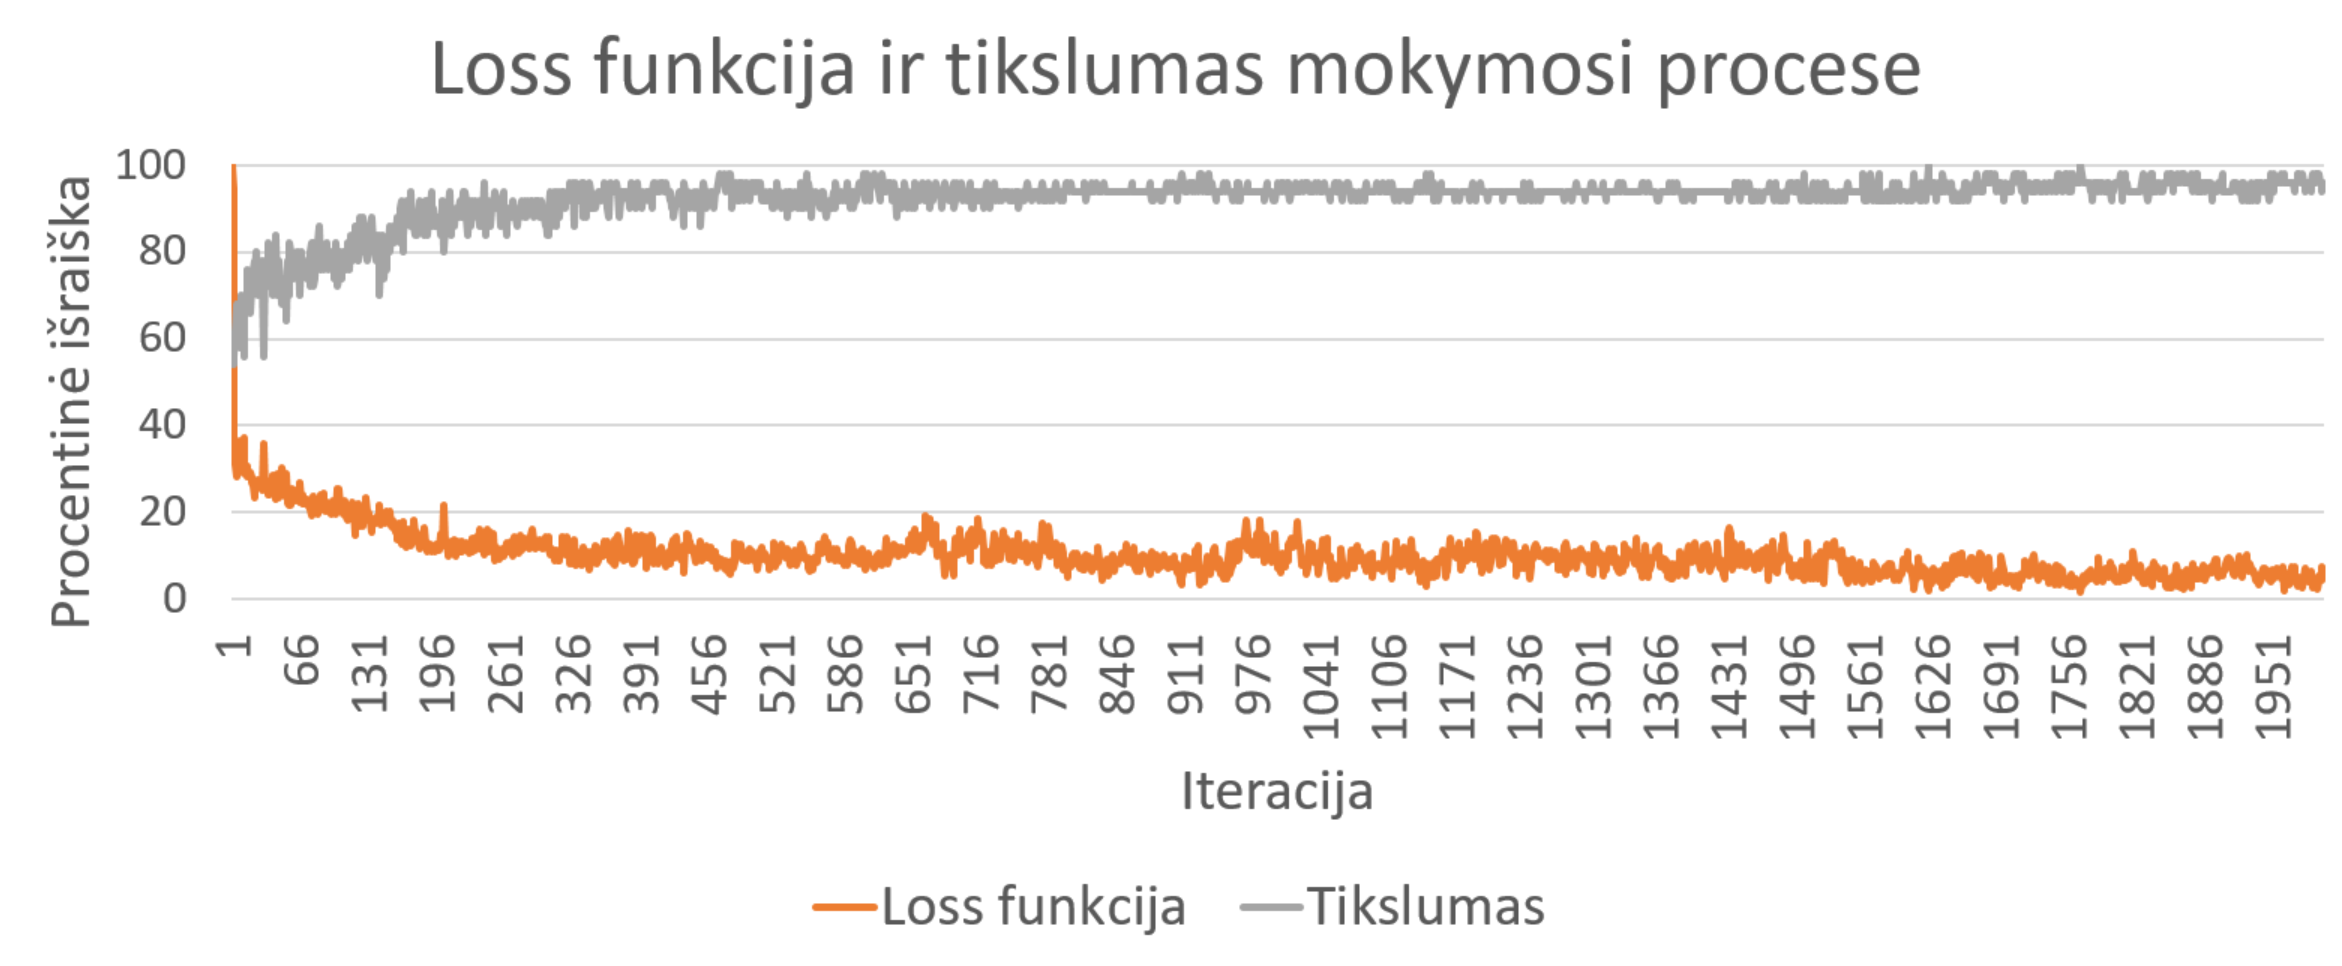
\includegraphics[width=14cm]{statistika.png}
  \captionof{figure}{Loss funkcijos ir tikslumo statistika mokymosi procese}
  \label{statistika}
\end{minipage}

Apmokymas buvo vykdomas su ASUS GeForce GTX 1070 8GB vaizdo plokšte. Apmokyti 100.000 paveikslėlių truko apytiksliai 4h. Vidutiniškai viena iteracija truko apytiksliai 7.2s (\ref{mokymas} pav.).
Paveikslėlių generavimas buvo vykdomas tuo pačiu metu naudojantis CPU.

\begin{minipage}{\linewidth}
  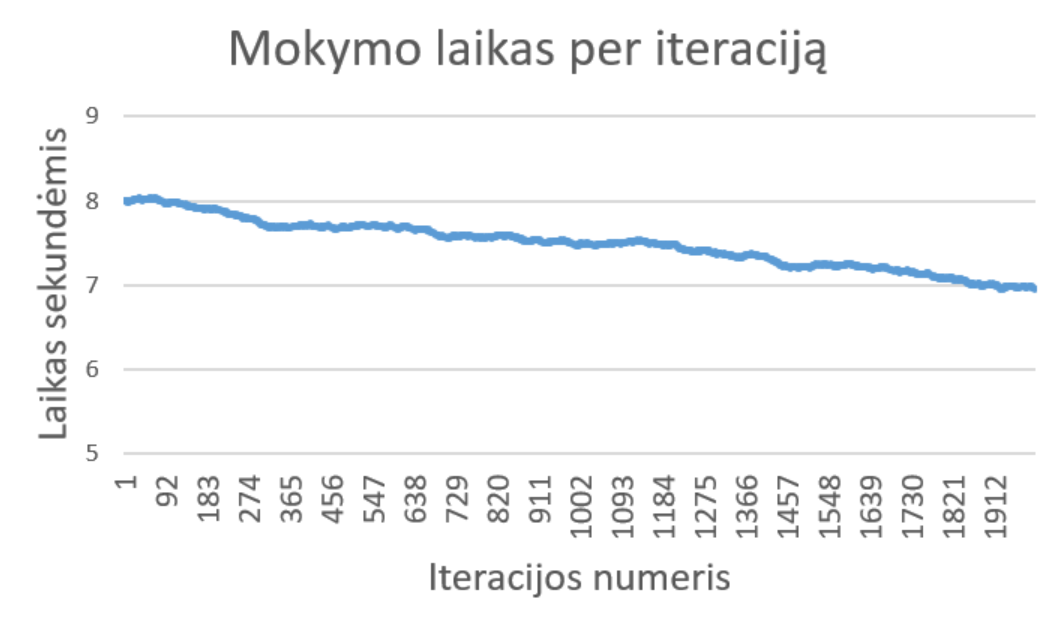
\includegraphics[width=12cm]{mokymas.png}
  \captionof{figure}{Neuroninio tinklo mokymo greitis}
  \label{mokymas}
\end{minipage}


\subsection{LSTM rekurentinio neuroninio tinklo mokymas}

Tesseract 4.00 versijoje pridėtas naujas atpažinimo variklis, kuris remiasi LSTM tipo rekurentiniu neuroniniu tinklu.
Lyginant su ankstesnėmis versijomis, ženkliai padidėjo dokumentų tipo nuotraukų teksto atpažinimas, tačiau tai reikalauja 
ženkliai didesnių kompiuterio skaičiavimo resursų. Atpažįstant sudėtingas kalbas, yra didelė tikimybė, kad atpažinimas truks 
greičiau nei bazinė pirminė Tesseract versija.

Naudojant neuroninius tinklus teksto atpažinimui yra reikalinga žymiai daugiau duomenų modelio treniravimui, taip pat pats 
treniravimas trunka ilgiau nei pirminėje Tesseract versijoje. Visoms lotynų rašmenimis pagrįstoms kalboms treniravimas vyko naudojant daugiau
nei 400.000 teksto eilučių bei apie 4.500 skirtingų šriftų. Su nauja versija ženkliai išaugo mokymosi laikas. Jei su ankstesne versija mokymas
trukdavo nuo kelių minučių iki kelių valandų, tai su nauja 4.00 versija tai gali trukti nuo kelių dienų iki kelių savaičių.
Tačiau ne visais atvejais yra naudinga treniruoti modelį nuo pradžių, priklausomai nuo situacijos, kartais užtenka pertreniruoti egzistuojantį modelį.

Išskiriami trys pagrindiniai modelio apmokymo principai:
\begin{itemize}[itemsep=0.5pt]
  \item Esamo modelio patobulinimas. Naudojant egzistuojantį pasirinktos kalbos modelį, papildomai apmokomas su papildomais specifiniais duomenimis.
  Tai gali išspręsti problemas, kai norimas rezultatas nedaug skiriasi nuo jau apmokyto modelio, pvz.: truputį nestandartinis šriftas.
  Gali veikti su sąlyginai mažu naujų duomenų kiekiu.
  \item Nuimti viršutinį (ar keletą daugiau) modelio sluoksnių ir pertreniruoti naujus sluoksnius su naujais duomenimis.
  Jei esamo modelio patobulinimas nesprendžia esamos problemos, šis būdas dažniausiai būna kitas pasirinkimas.
  Viršutinio sluoksnio permokymas vis dar gali veikti treniruojant visiškai naują kalbą, tačiau tos kalbos turi būti labai panašios, kad būtų pasiektas norimas efektas.
  \item Apmokymas nuo nulio. Tai gali būti labai sunki užduotis, jei nėra pakankamai daug reprezentatyvių duomenų spręsti konkrečiai problemai.
  Jei duomenų nėra pakankamai daug, galiausiai tinklas bus permokytas, kuris puikiai susidoros tik su mokymo duomenimis, tačiau visiškai neatliks savo užduoties,
  kai bus paduodami realūs duomenys. Nors mokymas atrodo skiriasi, matys treniravimo žingsniai yra beveik identiški aukščiau aprašytiems, taigi tai yra visai paprasta
  išbandyti, atsižvelgiant į turimų duomenų bei kompiuterio resursų kiekį.
\end{itemize}

\subsubsection{Atpažinimo kokybės gerinimas}
Egzistuoja įvairiausių priežasčių, kodėl Tesseract atpažinimo programa nesugeba atpažinti jai paduoto teksto.
Svarbu pabrėžti, kad Tesseract modelio permokymas retai padės, nebent naudojamas labai nestandartinis šriftas arba nauja dar netreniruota ir neapmokyta kalba.

\subsubsubsection{Paveikslėlio apdorojimas}
Pati Tesseract sistema savyje atlieka įvairius paveikslėlių apdorojimo veiksmus, pasinaudojant Leptonica biblioteka, prieš pradedant pati teksto atpažinimą.
Dažniausiai Tesseract puikiai susitvarko su šita užduotimi, tačiau neišvengiamai atsiranda situacijų, su kuriuomis automatiškai susidoroti nepavyksta ir dėl to pastebimai nukenčia
atpažinimo tikslumas.

Jei norima pamatyti, kaip Tesseract apdorojo paveiksliuką, tai galima atlikti pakeitus konfigūracinio parametro \textit{tessedtessedit\textunderscore write\textunderscore images} reikšmę į \textbf{true}
kai yra leidžiama Tesseract programa. Jei paruoštas tinklo apmokymui paveikslėlis atrodo problematiškai, neišvengiamai reikės pritaikyti viena ar daugiau paveikslėlių apdorojimo technikų
prieš siunčiant apdorojimui.

\textbf{Spalvų inversija}

Nors senesnės Tesseract versijos (<= 3.05) palaikė šviesų tekstą ant juodo fono be jokių problemų, nuo 4.00 versijos būtina sąlyga, kad tekstas būtų juodas, o fonas šviesus.
Tam tikslui atlikti užtenka vienos komandos:

\textbf{\textit{numpy.invert(image)}}

\textbf{Dydžio keitimas}

Tesseract programa geriausiai veikia, kai paduodamų paveikslėlių taškų viename colyje (angl. DPI) dydis yra bent 300, todėl labai svarbu užtikrinti, kad dydis nebūtų mažesnis.

Atliktas eksperimentas\footnote{\textit{Willus Dotkom} vartotojo atliktas eksperimentas. Šaltinis https://groups.google.com/forum/\#!msg/tesseract-ocr/Wdh\_JJwnw94/24JHDYQbBQAJ}
(žiūrėti \ref{tess4_error_rate} pav.) parodė, kad egzistuoja optimalus raidžių aukštis, kuriam esant klaidų tikimybė mažėja iki 0. Raidžių aukščiui esant tarp 30 ir 33 pikselių, klaidų tikimybė visiškai sumažėja,
todėl galima daryti prielaidą, kad labai svarbu pasirinkti tinkamą šrifto dydį ruošiant mokymo duomenis, norint pasiekti geriausių rezultatų.

\begin{minipage}{\linewidth}
  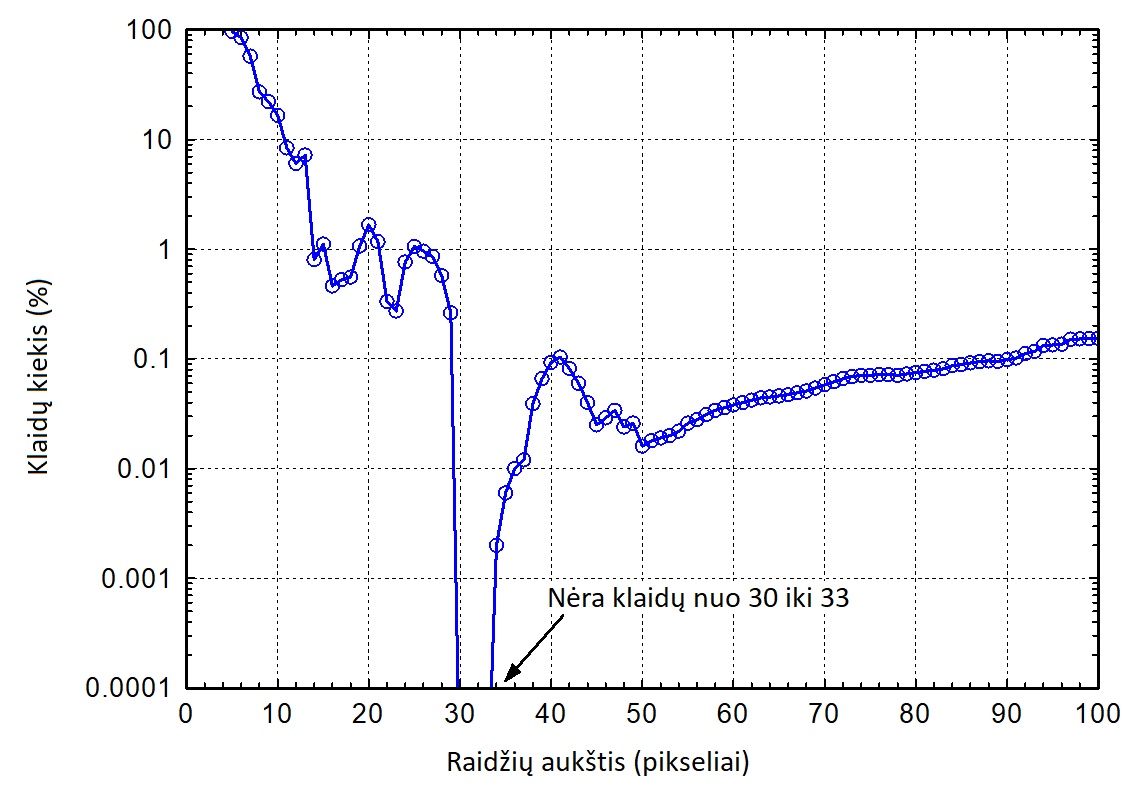
\includegraphics[width=12cm]{tess4_error_rate.png}
  \captionof{figure}{Klaidų kiekio priklausomybė nuo raidžių aukščio}
  \label{tess4_error_rate}
\end{minipage}
\textbf{Binarizacija}

Binarizacija - tai paveiksliuko spalvų keitimas į juodą ir baltą (\ref{binarisation} pav.). Tesseract jau turi integruotą funkcionalumą atlikti šiai užduočiai (naudojamas \textit{Otsu} algoritmas),
tačiau ne visada rezultatas gaunasi optimalus. Tai dažniausiai lemia netolygus fono tamsumas.

Jei nepavyksta išgauti geresnės kokybės nuotraukos, kuriame fono spalva būtų tolygi, yra alternatyvių ribinių verčių nustatymo algoritmų, kuriuos vertėtų išbandyti:
\begin{itemize}[itemsep=0.5pt]
  \item \textit{ImageJ} automatinis ribinių verčių nustatymo algoritmas (JAVA programavimo kalba).
  \item \textit{OpenCV} ribinių verčių nustatymo algoritmas (Python programavimo kalba).
  \item \textit{scikit-image} ribinių verčių nustatymo algoritmas (Python programavimo kalba).
\end{itemize}

\begin{minipage}{\linewidth}
  \centering
  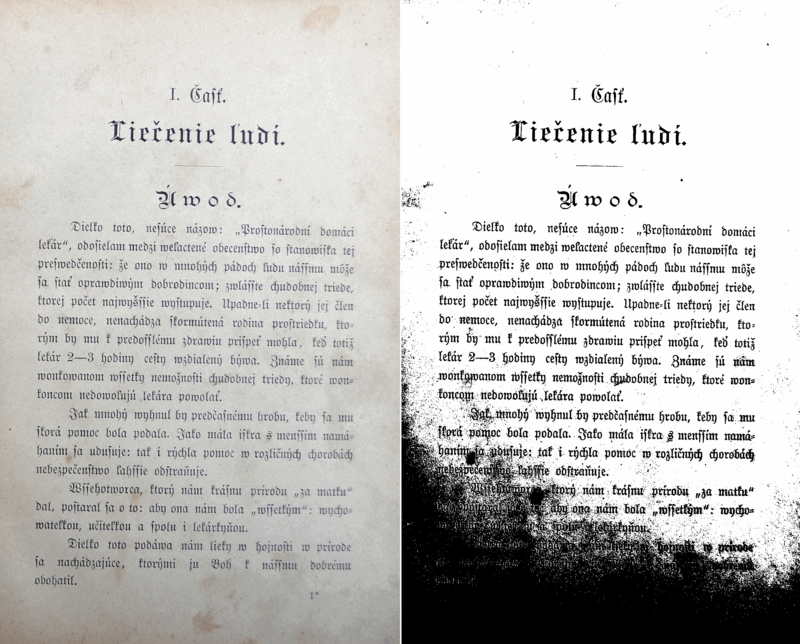
\includegraphics[width=10cm]{binarisation.png}
  \captionof{figure}{Binarizacijos algoritmo taikymo rezultatas}
  \label{binarisation}
\end{minipage}

\textbf{Triukšmo pašalinimas}

Triukšmas - tai atsitiktinis netolygaus ryškumo išsibarstymas paveikslėlyje, kuris gali padaryti tekstą sunkiai ar visai neįskaitomu (\ref{noise} pav.).
Yra specifiniai triukšmo tipai, kurių Tesseract nesugeba pašalinti vykdydama binarizacijos etapą, todėl ženkliai sumažėja atpažinimo tikslumas.

\begin{minipage}{\linewidth}
  \centering
  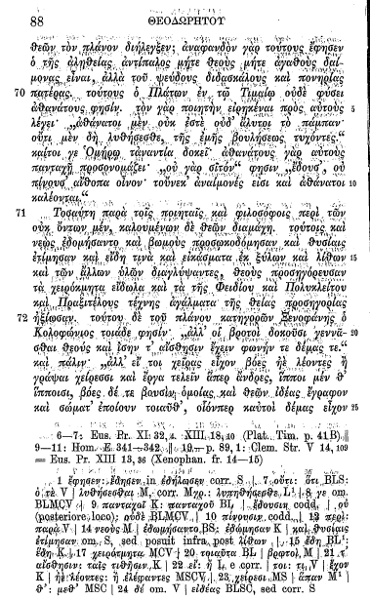
\includegraphics[width=10cm]{noise.png}
  \captionof{figure}{Pašalintas triukšmas}
  \label{noise}
\end{minipage}

\textbf{Pasukimas / Iškreipimas}

Iškreiptas paveikslėlis būna tada, kai yra nuskanuojamas lapas kreivai (\ref{skew-linedetection} pav.). Tesseract linijų atpažinimo tikslumas sumažėja jei puslapis nėra visiškai horizontalus, o
tai įtakoja patį teksto atpažinimą. Norint išspręsti šią problemą, reikia pakreipti puslapį taip, kad tekslo linijos būtų horizontalios.

\begin{minipage}{\linewidth}
  \centering
  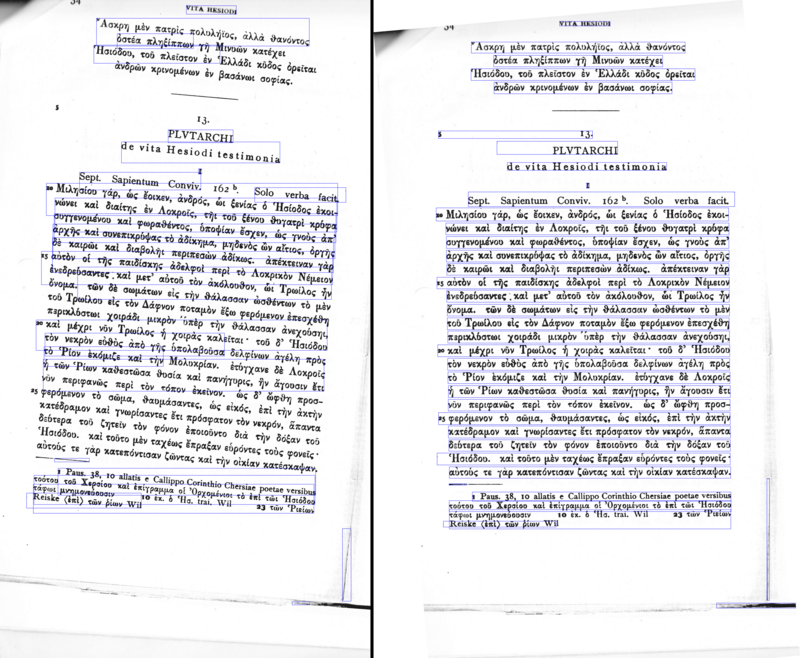
\includegraphics[width=10cm]{skew-linedetection.png}
  \captionof{figure}{Iškreipto puslapio išlyginimas}
  \label{skew-linedetection}
\end{minipage}

\textbf{Skanuotų puslapių kraštinių naikinimas}

Skanuoti puslapiai dažnai turi tamsias kraštinės aplinkui tekstą (\ref{borders} pav.). 
Tai dažnai gali būti atpažįstami kaip papildomi simboliai, ypač jei skiriasi jų formos ir atspalviai.

\begin{minipage}{\linewidth}
  \centering
  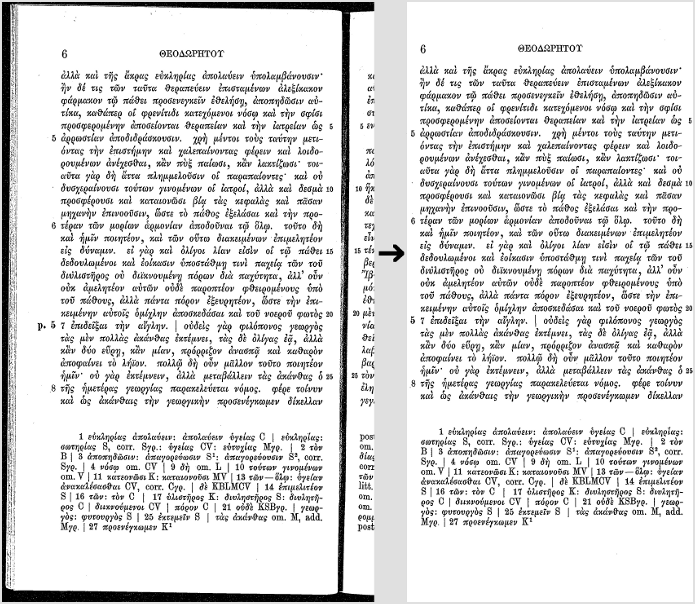
\includegraphics[width=10cm]{borders.png}
  \captionof{figure}{Puslapio kraštinių naikinimas}
  \label{borders}
\end{minipage}

\textbf{Tekstas be kraštinių}

Jei norimas atpažinti tekstas visiškai neturių kraštinių ir yra nuo krašto iki krašto, Tesseract programa gali turėti sunkumų bandant atpažinti tekstą.
Panaudojant vieną komandą, lengvai galima pridėti kraštines iš visų pusių (naudojama \textit{ImageMagick®} programa):

\textbf{\textit{convert  input.jpg  -bordercolor White -border 10x10 output.jpg}}

\textbf{Permatomumas / alfa kanalas}

Kai kurie paveikslėlių formatai (pvz.: png) turi alfą kanalą, kuris suteikia galimybę saugoti permatomumo reikšmę nuotraukoje.
Alfa kanalu dažniausiai nusakomas paveikslėlio skaidrumas. Paprastai prie 24 nuotraukos bitų, kuriuose kiekvienai iš trijų pagrindinių spalvų skiriama po 8 bitus, pridedami papildomi
8 bitai, kurie saugo skaidrumo informaciją. 

Tesseract 3.0x versijos tikisi, kad pats vartotojas pateiks paveiksliuką jau su panaikinta alfa kanalu. Tai gali būti padaroma su tokia komanda (naudojama \textit{ImageMagick®} programa):

\textbf{\textit{convert input.png -alpha off output.png}}

Tesseract 4.00 versijoje yra funkcionalumas, kuris pats pašalina alfa kanalą naudojant \textit{Leptonica} programos komandą \textit{pixRemoveAlpha()}. Ši komanda panaikina alfa kanalą
suliedama jį su baltu fonu. Kartais (pvz.: filmų subtitrų atpažinimas) tai gali sukelti problemų, todėl vartotojai turėtų patys panaikinti alfa kanalą arba pritaikyti spalvų inversiją.

\subsubsubsection{Puslapių skirstymo metodas}
Tesseract programos standartinis veikimo principas pagrįstas tuo, kad programa tikisi paveikslėlio puslapio
pavidalu su jame esančiu tekstu. Tačiau, jei norima atpažinti tik dalį teksto, yra įvairiausių teksto skirstymo 
parametrų, kurį reikia nurodyti naudojant komandą \textit{--psm} ir nurodant komandos numerį.

\begin{enumerate}[itemsep=0.5pt]
  \setcounter{enumi}{-1}
  \item Orientacija ir rašto aptikimas (OSD).
  \item Automatinis puslapio skirstymas su rašto aptikimu (OSD).
  \item Automatinis puslapio skirstymas, bet be rašto aptikimo (OSD) ir be simbolių atpažinimo (OCR).
  \item Pilnai automatinis puslapio skirstymas, bet be rašto aptikimo (OSD) (Numatytasis režimas).
  \item Vienas teksto stulpelis.
  \item Vienas vertikaliai išlygiuoto teksto blokas.
  \item Vienas teksto blokas.
  \item Paveikslėlį laikyti kaip vieną teksto liniją.
  \item Paveikslėlį laikyti kaip vieną žodį.
  \item Paveikslėlį laikyti kaip vieną žodį apskritime.
  \item Paveikslėlį laikyti kaip vieną simbolį.
  \item Išmėtytas tekstas. Rasti kuo daugiau teksto nesilaikant jokios tvarkos.
  \item Atpažinti išmėtytą tekstą su rašto aptikimu (OSD).
  \item Neapdorota eilutė. Paveikslėlį laikyti kaip vieną teksto liniją, išvengiant specifinių Tesseract gudrybių.
\end{enumerate}

\subsubsubsection{Žodynai, žodžių sąrašai, šablonai}
Tesseract programa optimizuota taip, kad geriausiai atpažintų sakinius, susidarančius iš žodžių. 
Jei yra bandoma atpažinti nestandartinės strukturos tekstus (pvz.: sąskaitas, čekius, prekių sąrašus, kodus), yra keletas papildomų 
būdų, kaip būtų galima pagerinti atpažinimo tikslumą.

Pirmiausiai reikia įsitikinti, kad yra pasirinktas tinkamas puslapio skirstymo būdas. Tai užtikrina, kad bus efektyviausiai ieškoma teksto.

Žodynų atjungimas, kuriuos naudoja Tesseract turėtų pagerinti atpažinimą, jei dauguma teksto nėra žodyne esantys žodžiai.
Norint išjungti funkcionalumą, kai naudojami Tesseract žodynai, reikia nurodyti \textit{FALSE} reikšmę šiems konfigūraciniams parametrams:
\textit{load\textunderscore system\textunderscore dawg} ir \textit{load\textunderscore freq\textunderscore dawg}.

Taip pat yra galimybė pačiam vartotojui prisidėti norimus žodžius į Tesseract programą, kurie padės atpažinimo varikliui geriau suprasti žodžius.
Be žodžių, yra galimybė prisidėti simbolių sekų šablonus, kurie dar labiau padės pagerinti tikslumą.

\subsubsection{Rinkmenų pasiruošimas}
Bendrai mokymo žingsniai yra tokie:

\begin{enumerate}[itemsep=0.5pt]
  \item Pasiruošti norimą apmokyti tekstą.
  \item Sugeneruoti paveiksliuką su tekstu + \textit{box} failu.
  \item Sukurti \textit{unicharset} failą.
  \item Iš \textit{unicharset} sukurti pradinę apmokymo duomenų failą ir nebūtiną žodynų informaciją. 
  \item Paleisti \textit{Tesseract}, kad apdorotų paveikslėlį ir \textit{box} failą bei sukurtų apmokymo duomenų rinkinį.
  \item Paleisti treniravimą su sukurtu duomenų rinkiniu.
  \item Sujungti duomenų failus.
\end{enumerate}

Norint atlikti LSTM rekurentinio tinklo mokymą Tesseract 4.0 versijos aplinkoje, reikia susigeneruoti atitinkamo formato mokymo rinkmenas.
Kiekvienas sugeneruotas automobilio numeris turi turėti 5 skirtingus rinkmenas:
\begin{itemize}[itemsep=0.5pt]
  \item .box formato - rinkmena, kurią sugeneruoja priede \ref{generate_line_box} pridėta programa.
  \item .lstmf formato - rinkmena, kurią sugeneruoja priedo \ref{makefile} komanda: lists. 
  \item .gt.txt formato - tekstinė rinkmena, kurioje yra tekstas, kuris yra pavaizduotas paveikslėlyje.
  \item .txt formato - rinkmena, kurią sugeneruoja priedo \ref{makefile} komanda: lists. 
  \item .tif formato - paveiksliukas, išsaugotas TIFF formatu.
\end{itemize}

\subsubsection{Modelio apmokymas}

Norint paleisti modelio apmokymą, reikia paleisti komandą: 

\textbf{\textit{make training MODEL\_NAME=modelis}}

Ši komanda yra trumpinys pilnos komandos:

\textbf{\textit{make unicharset lists proto-model training MODEL\_NAME=modelis}}

Vykdomos operacijos:
\begin{itemize}[itemsep=0.5pt]
  \item \textit{unicharset} - Sukurti galimų simbolių sąrašą.
  \item \textit{lists} - Sukurti sąrašą \textit{.lstmf} failų ir išskirstyti juos į treniravimo ir verifikavimo.
  \item \textit{training} - Pradėti mokymą.
  \item \textit{proto-model} - Sugeneruoti modelį.
\end{itemize}

\subsubsection{Mokymo statistika}
Vykdant neuroninio tinklo apmokymą su maksimaliai 10.000 iteracijų, buvo pasiekti žemiau pavaizuoti rezultatai.
Vieno simbolio atpažinimo klaidų kiekį mokymo metu galima pamatyti \ref{char_stats} pav.
Vieno žodžio atpažinimo klaidų kiekį mokymo metu galima pamatyti \ref{word_stats} pav.

\begin{minipage}{\linewidth}
  \centering
  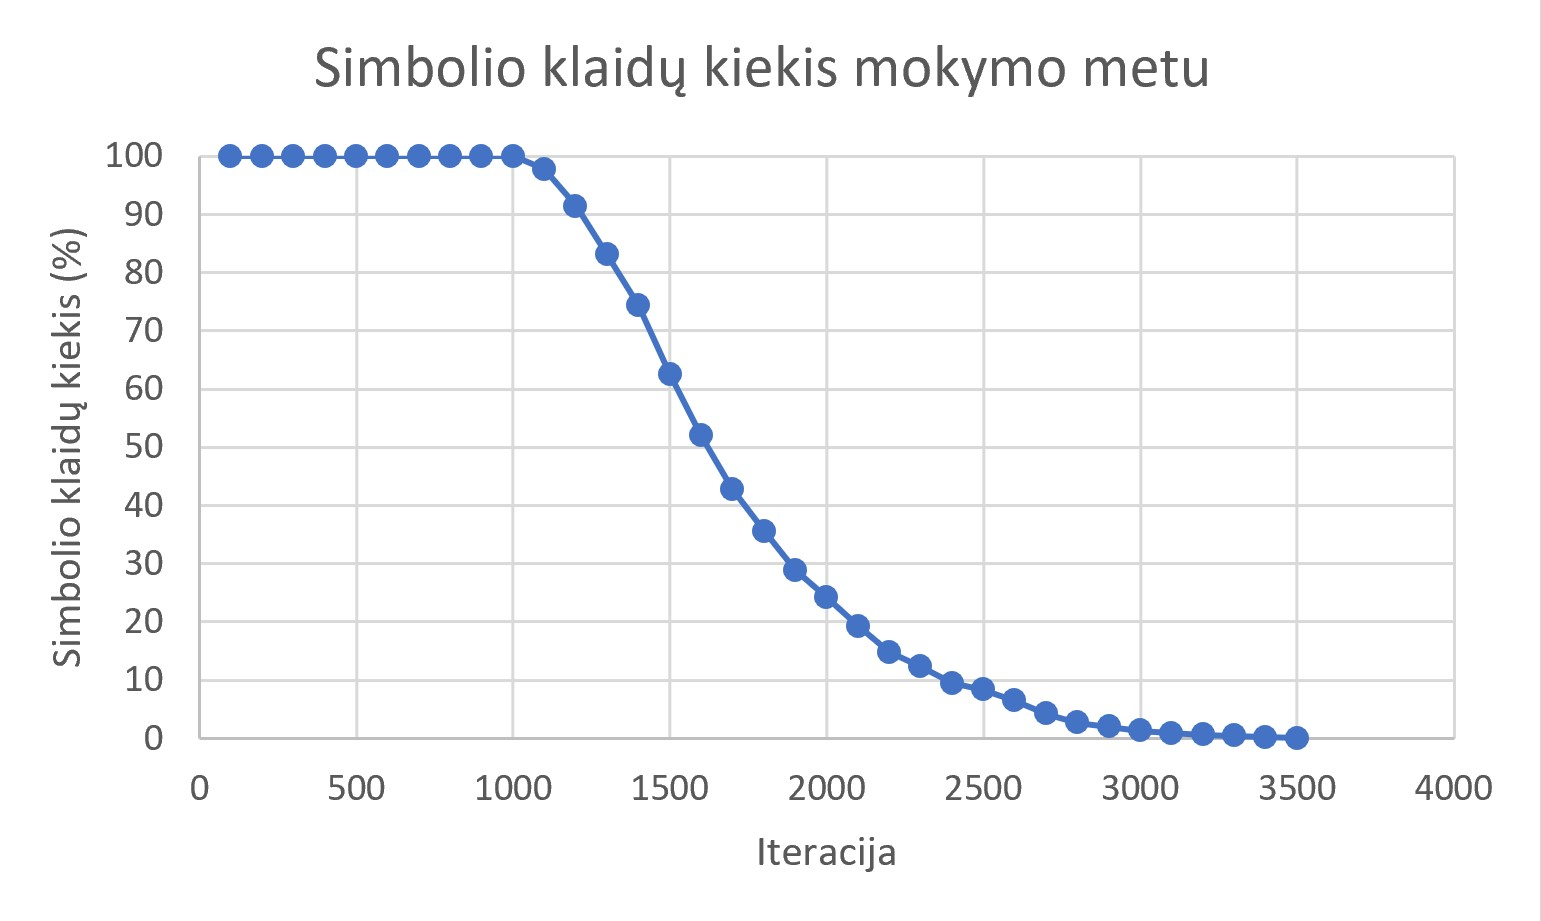
\includegraphics[width=12cm]{char_stats.jpg}
  \captionof{figure}{Simbolio klaidų kiekis mokymo metu}
  \label{char_stats}
\end{minipage}

\begin{minipage}{\linewidth}
  \centering
  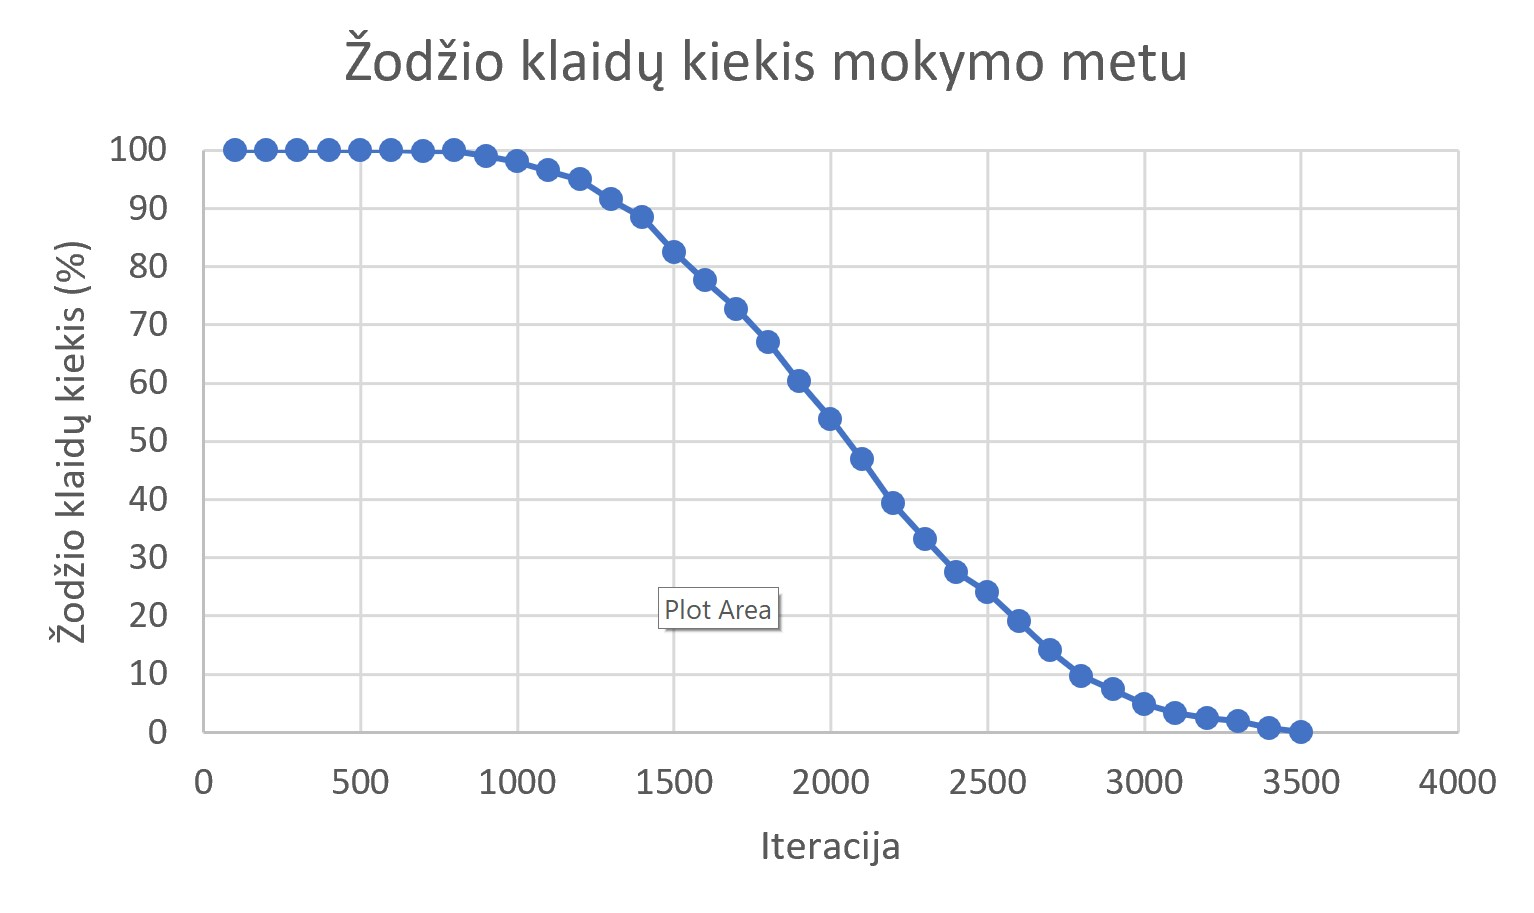
\includegraphics[width=12cm]{word_stats.jpg}
  \captionof{figure}{Žodžio klaidų kiekis mokymo metu}
  \label{word_stats}
\end{minipage}





\pagebreak
\section{Vaizdo atpažinimas}
Šiame skyriuje aprašoma kaip panaudojami apmokyti neuroniniai tinklai skirti atlikti jiems paskirtas užduotis.

\subsection{Numerio rėmelio atpažinimas}
Norint aptikti ir atpažinti realiuose paveikslėliuose numerio rėmelį, į neuroninį tinklą paduodamos 128x64 pikselių dydžio
paveikslėlio dalys, kaip jau buvo aprašyta \ref{Mokymo duomenų generavimas} skyriuje.
Atpažįstant realius paveikslėlius, naudojama kitokia neuroninio tinklo architektūra. Paskutiniai du lygmenys vietoj to, 
kad būtų pilnai sujungti, yra konvoliuciniai. Taip pat pradinio paveikslėlio dydis neturi būti 128x64 pikselių, o gali būti
bet koks. Idėja tokia, kad pilno dydžio paveikslėlis gali būti paduodamas į neurorinį tinklą suskaidant jį į dalis slenkančio
langelio principu, bei kiekvienai iš jų grąžinant rezultatą, ar rėmėlis egzistuoja. Naudojant vienodą neuroninį tinklą visoms 
paveikslėlio dalims yra pranašesnis nei atskiri neuroniniai tinklai, kadangi slenkantys langai dalinsis dauguma konvoliucinių 
savybių tarpusavyje, todėl nereikės kiekvieną kart atlikti naujų skaičiavimo operacijų.

Slenkančio lango principu veikiančio neuroninio tinklo rezultatai:

\begin{minipage}{\linewidth}
  \centering
  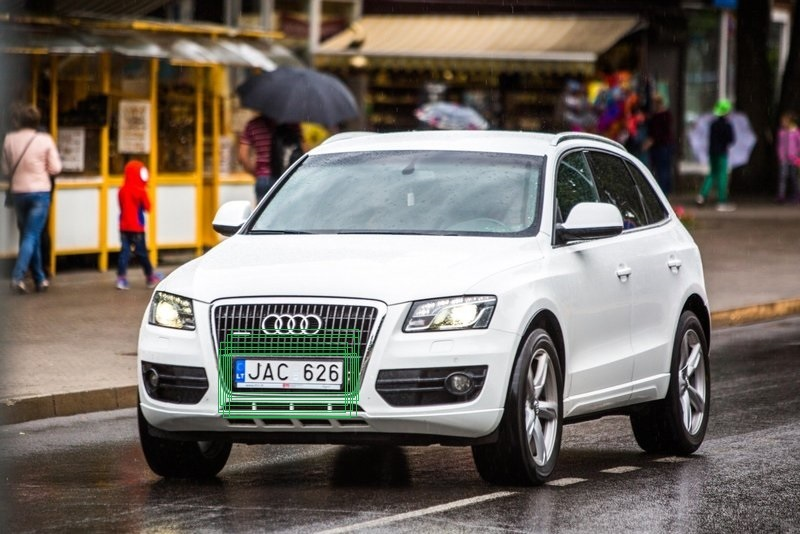
\includegraphics[width=12cm]{sliding.jpg}
  \captionof{figure}{Slenkančio lango principu gauti rezultatai}
  \label{daug_remeliu}
\end{minipage}

Žali stačiakampiai (\ref{daug_remeliu} pav.) vaizduoja regionus kur tikimybė, kad rėmelis egzistuoja yra didiesnė arba lygi 99\%.
Tai padaryta tokiu tikslu, kadangi mokymo duomenų aibėje apie 50\% paveikslėlių yra su egzistuojančiu numerio rėmeliu,
kai realiame pasaulyje paveikslėlių su numerio rėmeliais yra daug mažiau. Jeigu būtų naudojama 50\% tikimybė atrinkti 
teisingiems paveikslėliams, tai būtų neapsisaugota nuo pasitaikančių panašių paveikslėlių atitikmenų.

Norint panaikinti perteklinius dublikatus, pritaikomas 
Non-Maximum Suppresion \footnote{Non-Maximum Suppresion angl. - ne maksimalios reikšmės slopinimo algoritmas} algoritmas, kuris
tarp visų besikertančių stačiakampių palieka tik didžiausią tikimybę turinčią reikšmę\cite{girshick2014rich}.

Gavus likusį vieną stačiakampį (\ref{cropped} pav.), pagal to objekto koordinates iškerpamas paveikslėlis ir gaunamas toks rezultatas:

\begin{minipage}{\linewidth}
  \centering
  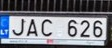
\includegraphics[width=4cm]{cropped_4.jpg}
  \captionof{figure}{Iškirptas gautas rezultatas}
  \label{cropped}
\end{minipage}



\subsection{Numerio simbolių atpažinimas}
Sukurta programa, kuri naudodama apmokytą LSTM pagrindu veikiantį neuroninį tinklą atpažįsta automobilio numerius (žiūrėti priede \ref{detect}).

Atpažinimo pavyzdžius galima pamatyti \ref{DGZ473} pav., \ref{EV0741} pav., \ref{FON550} pav., \ref{JPC320} pav., \ref{KTP049} pav., \ref{KZF273} pav., \ref{LAN285} pav.

Pavyzdžiai:
\newline
\begin{subfigure}{\linewidth}
  \centering
  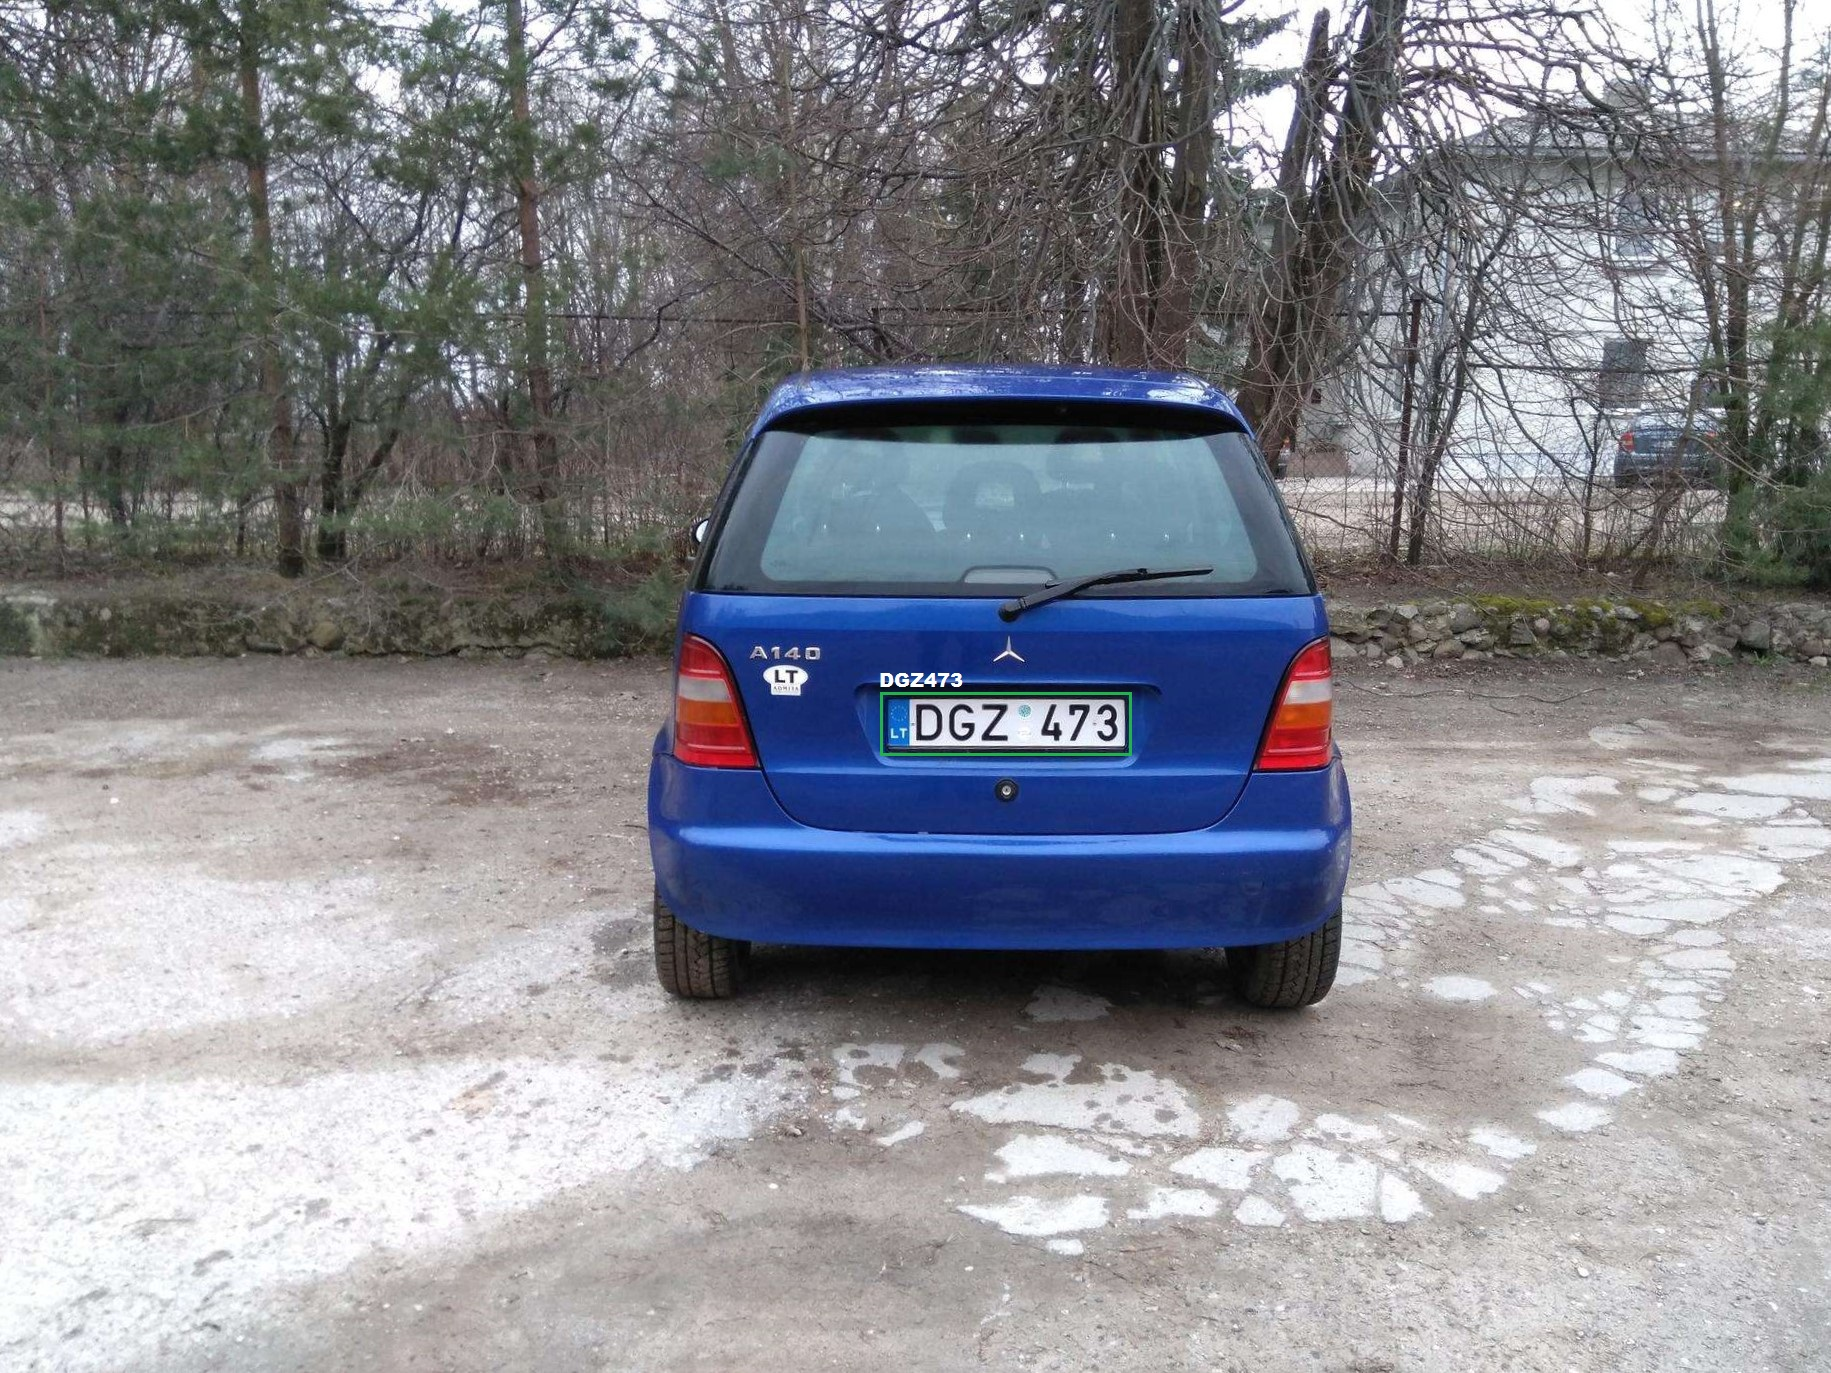
\includegraphics[width=6cm]{cars/dgz473.jpg}
  \captionof{figure}{Tikimasis rezultatas \textbf{DGZ473}.}
  \label{DGZ473}
\end{subfigure}
\begin{subfigure}{\linewidth}
  \centering
  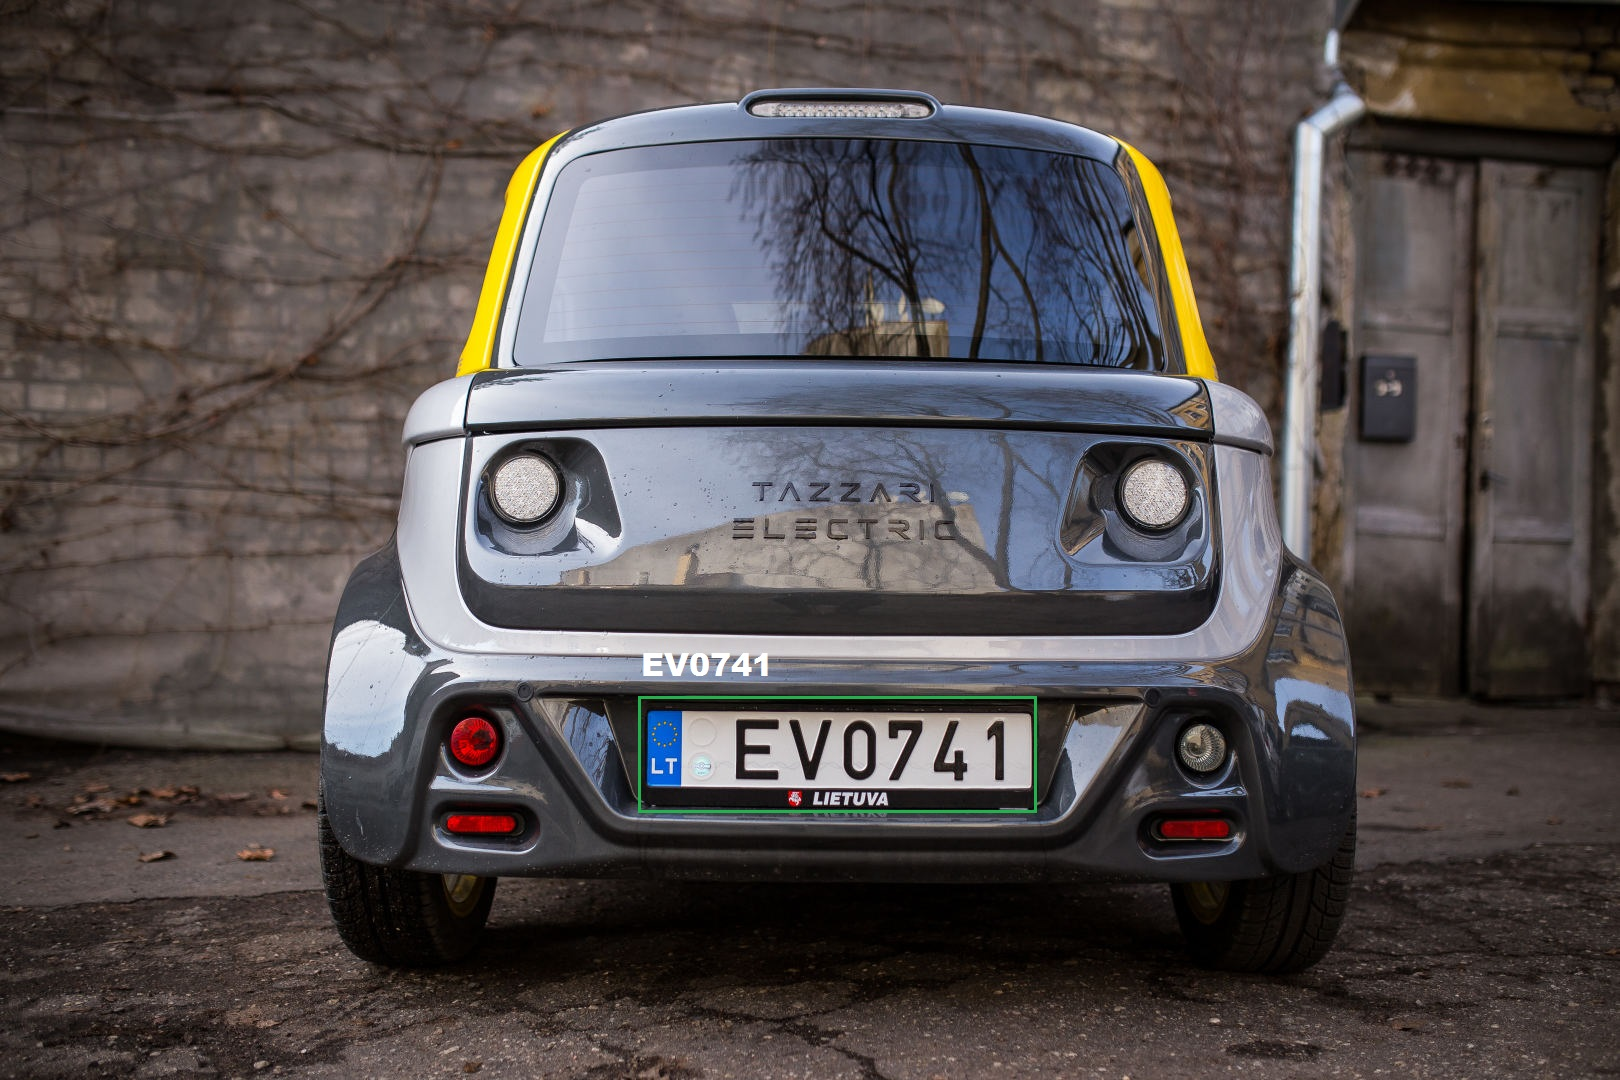
\includegraphics[width=6cm]{cars/ev0741.jpg}
  \captionof{figure}{Tikimasis rezultatas \textbf{EV0741}.}
  \label{EV0741}
\end{subfigure}
\begin{subfigure}{\linewidth}
  \centering
  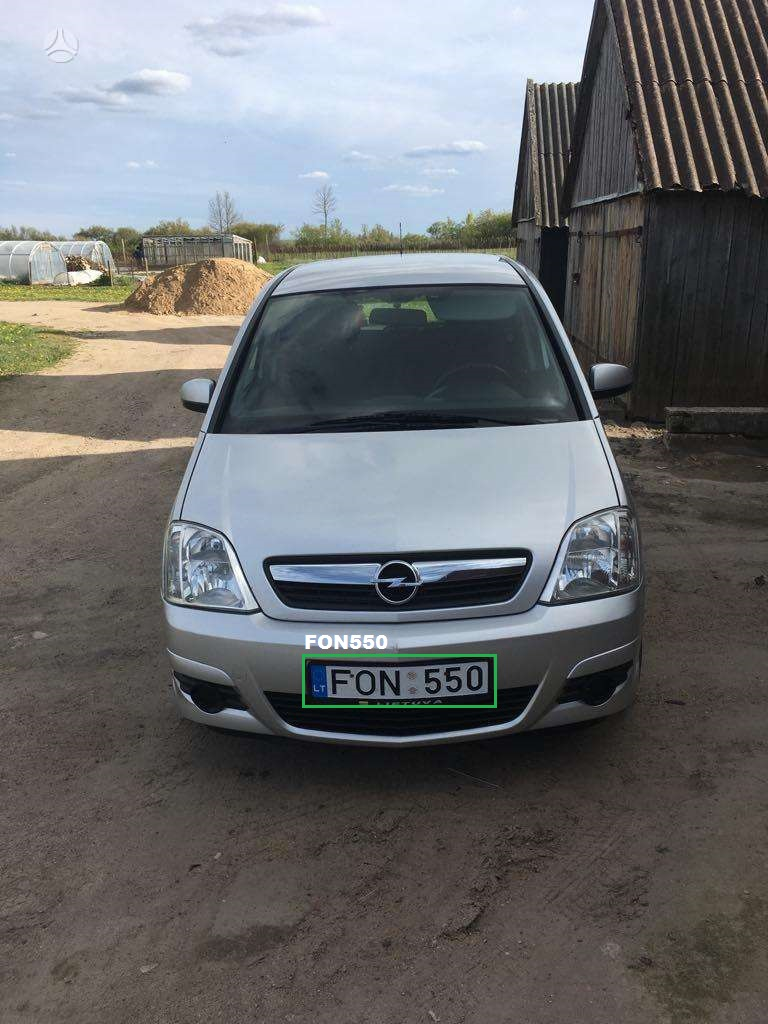
\includegraphics[width=6cm]{cars/fon550.jpg}
  \captionof{figure}{Tikimasis rezultatas \textbf{FON550}.}
  \label{FON550}
\end{subfigure}
\begin{subfigure}{\linewidth}
  \centering
  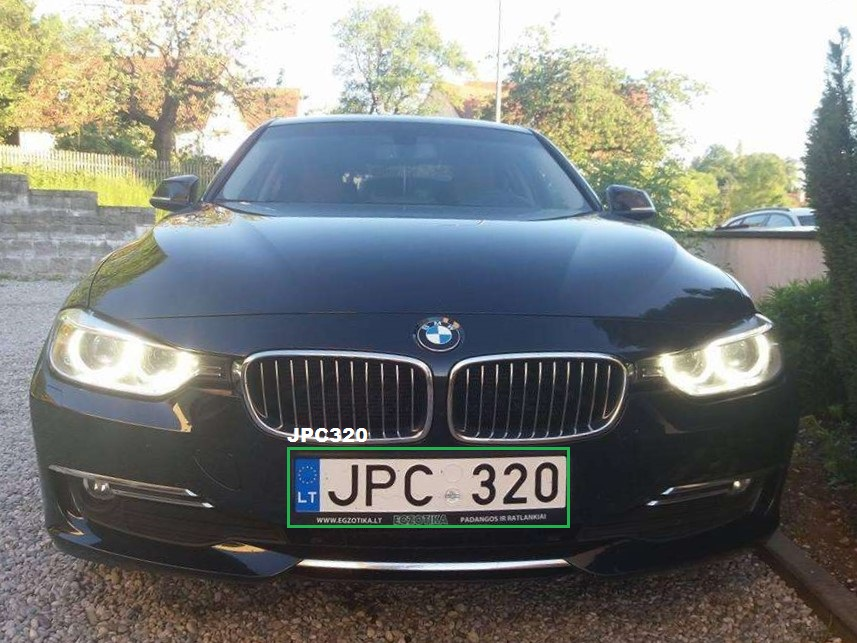
\includegraphics[width=6cm]{cars/jpc320.jpg}
  \captionof{figure}{Tikimasis rezultatas \textbf{JPC320}.}
  \label{JPC320}
\end{subfigure}
\begin{subfigure}{\linewidth}
  \centering
  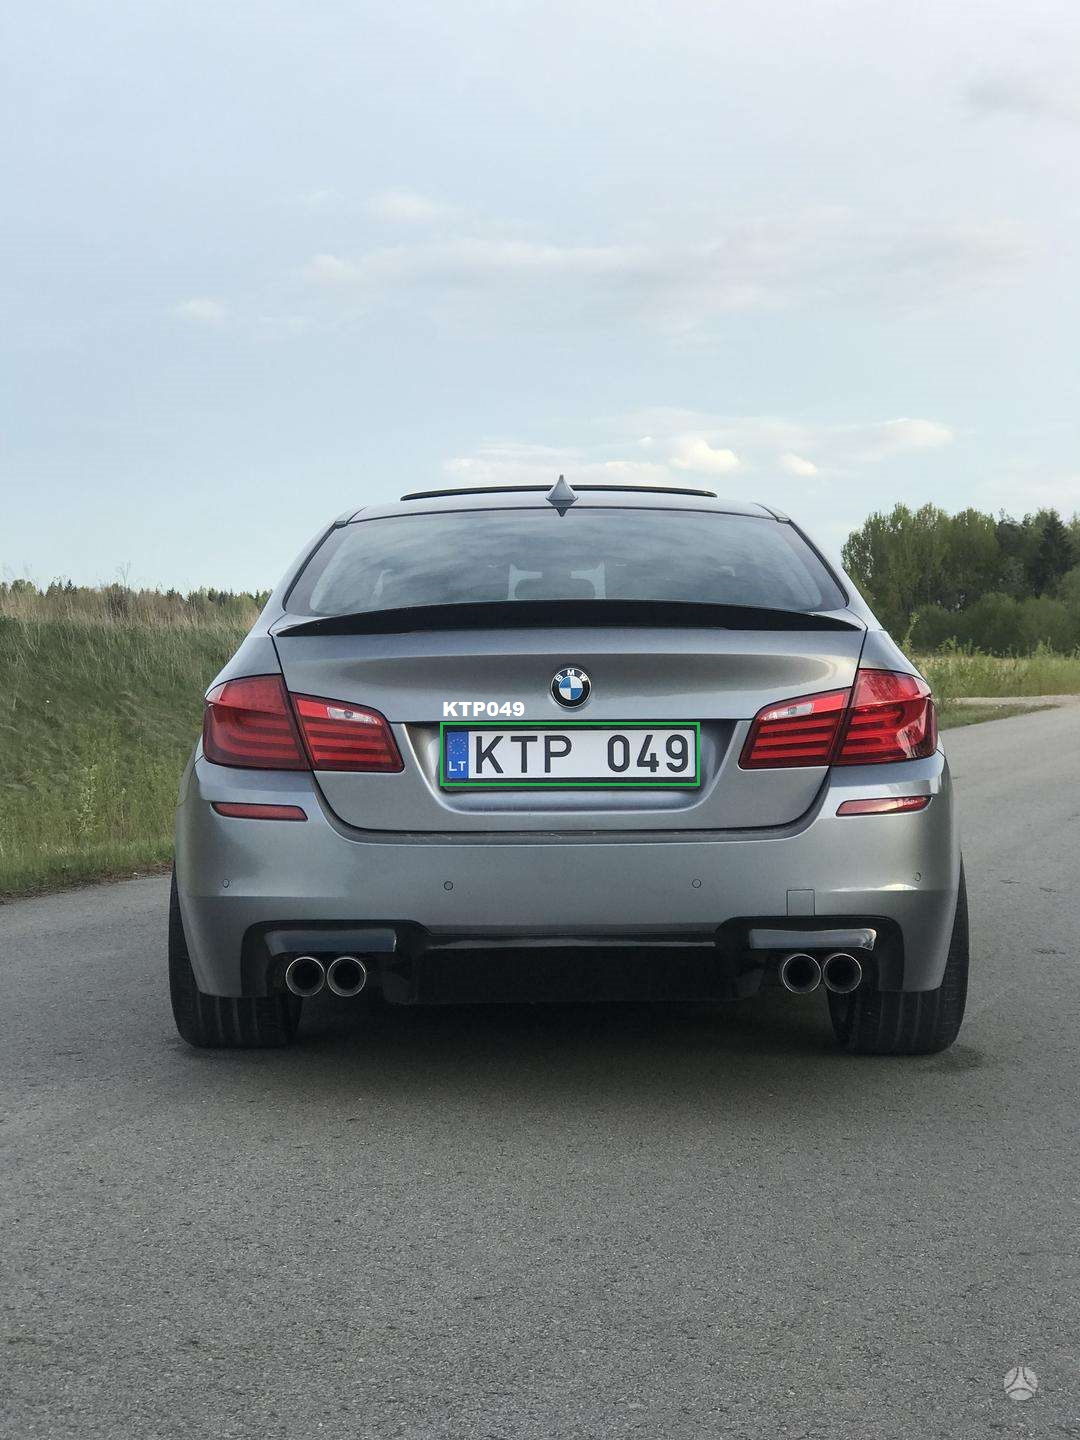
\includegraphics[width=6cm]{cars/ktp049.jpg}
  \captionof{figure}{Tikimasis rezultatas \textbf{KTP049}.}
  \label{KTP049}
\end{subfigure}
\begin{subfigure}{\linewidth}
  \centering
  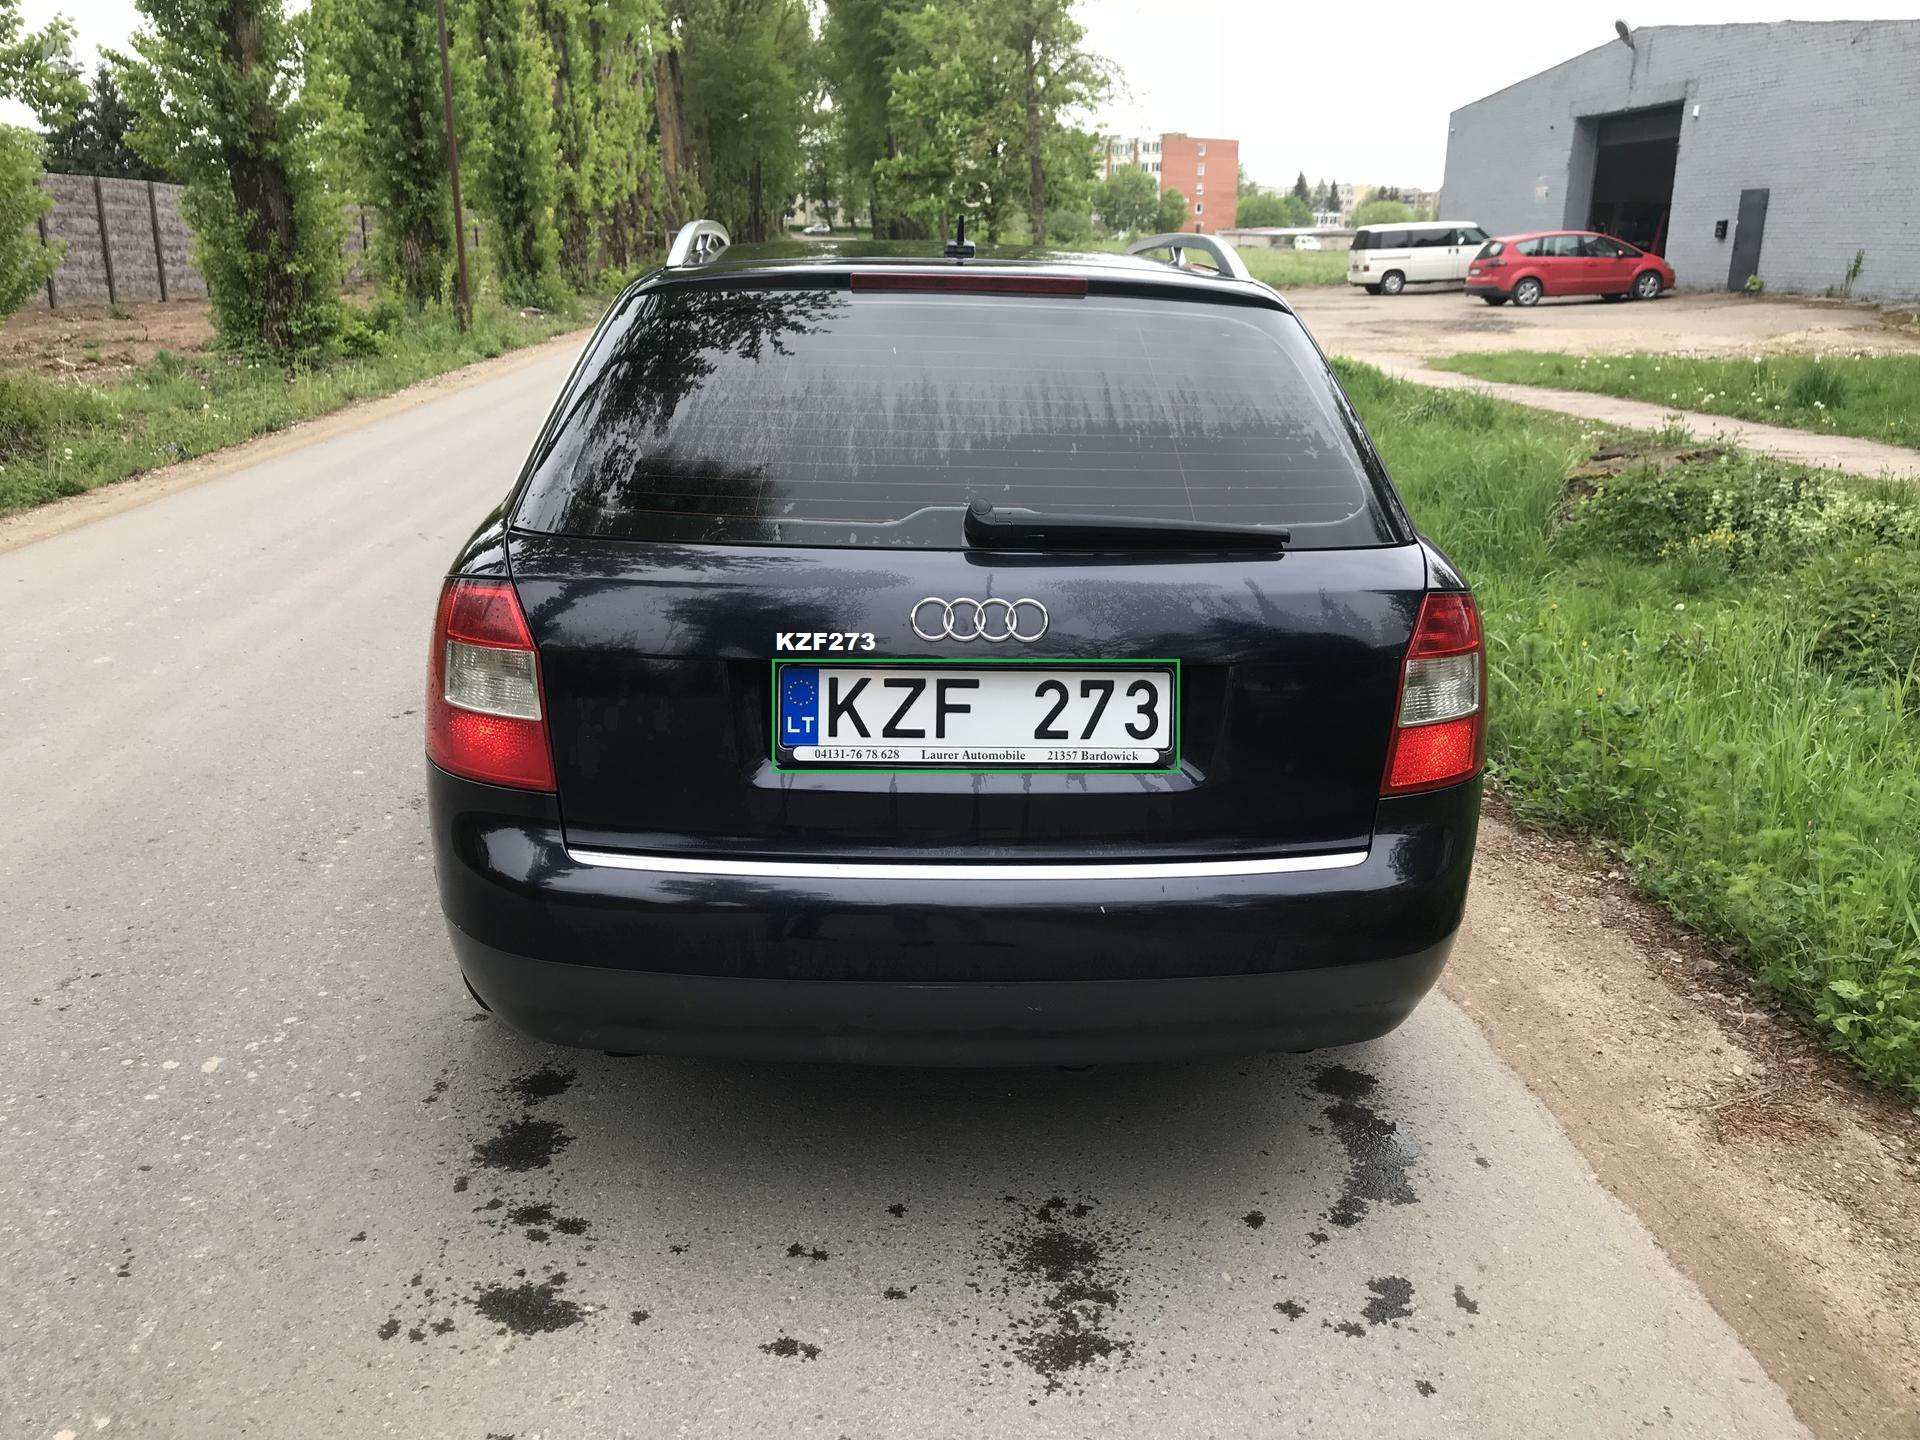
\includegraphics[width=6cm]{cars/kzf273.jpg}
  \captionof{figure}{Tikimasis rezultatas \textbf{KZF273}.}
  \label{KZF273}
\end{subfigure}
\begin{subfigure}{\linewidth}
  \centering
  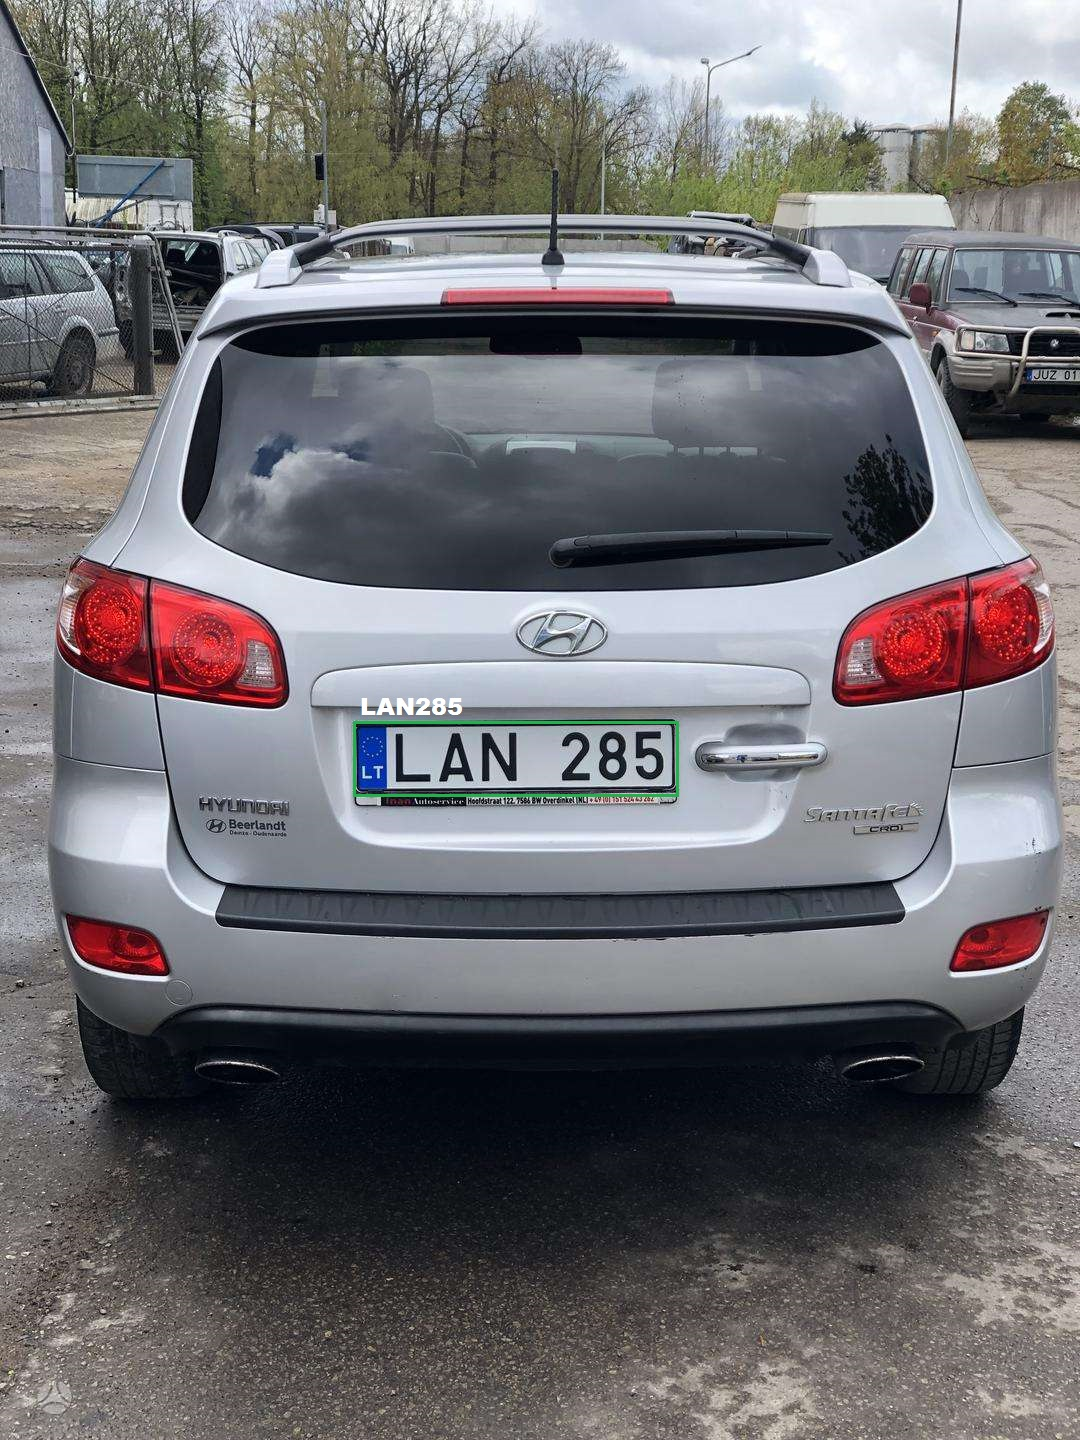
\includegraphics[width=6cm]{cars/lan285.jpg}
  \captionof{figure}{Tikimasis rezultatas \textbf{LAN285}.}
  \label{LAN285}
\end{subfigure}



\pagebreak
\sectionnonum{Rezultatai}
\begin{enumerate}[itemsep=0.5pt]%[itemsep=0.5pt]
  \item Sugeneruota 100.000 paveikslėlių, skirtų apmokyti neuroninį tinklą.
  \item Apmokytas kursinio darbo metu sukurtas neuroninis tinklas su 100.000 sugeneruotų paveikslėlių.
  \item Apmokytas modifikuotas Tesseract LSTM rekurentinis neuroninis tinklas panaudojant sugeneruotus paveikslėlius.
  \item Parašyta programa, kuri gauna rėmelio koordinates iš paveikslėlio, kuriame yra numeris, pasinaudojus neuroniniu tinklu.
  \item Parašyta programa, kuri iškerpa rėmelį pagal koordinates ir pasinaudojus modifikuotu Tesseract LSTM rekurentiniu neuroniniu tinklu atpažįsta numerį bei atvaizduoja pradiniame paveikslėlyje.
  \item Tinklas ištestuotas su tikrais paveikslėliais, kuriose yra lietuviški automobilių numeriai.
\end{enumerate}

\sectionnonum{Išvados}
Darbe buvo nagrinėta kaip išspręsti vaizdo atpažinimo problemą naudojantis neuroniniais tinklais.
Atlikus eksperimentą buvo gautos šios išvados:
\begin{enumerate}[itemsep=0.5pt]
  \item Pavyko atpažinti automobilių numerius naudojantis konvoliuciniu neuroniniu tinklu.
  \item Sukurto neuroninio tinklo pasiekta sparta (vid. 3 sekundės) nėra pakankama fiksuoti visų automobilių numerius stebint tiesioginiu vaizdu, tačiau yra pakankama integravus sistemą į stovėjimo aikštelių užkardus.
  \item Programa atpažįsta tik tuos numerius, kurie nėra daugiau nei 15\% pakrypę.
  \item Programa atpažįsta tik tuos numerius, kurių formatas yra trys raidės ir trys skaičiai.
  \item Mokant rekurentinį neuroninį tinklą didelę neigiamą įtaką tikslumui daro paveikslėlių iškrypimai.
  \item Prieš siunčiant paveikslėlį į rekurentinį neuroninį tinklą reikia jį apdoroti pagal rekomendacijas, kad paveikslėlis būtų atpažintas.
  \item Naudojant rekurentinį neuroninį tinklą simbolių atpažinimas vyksta sparčiau nei kiti išbandyti OCR įrankiai.
  \item Naudojant rekurentinį neuroninį tinklą atpažinimo tikslumas gali būti didesnis nei skandartinių OCR įrankių, jei modelis yra tinkamai apmokytas.
\end{enumerate}
\pagebreak
\printbibliography[heading=bibintoc]

\pagebreak
\sectionnonum{Sąvokų apibrėžimai}
\begin{itemize}[itemsep=0.5pt]
  \item Tesseract - optinė ženklų atpažinimo programa, kuri geba naudoti neuroninius tinklus atpažinimui.
  \item Leptonica - atviro kodo programinė įranga, skirta dirbti su paveikslėliais.
  \item Tensorflow - atviro kodo matematinė programinė įranga, naudojama darbui su neuroniais tinklais.
  \item OpenMP - programavimo standartas, skirtas realizuoti lygiagretiesiems algoritmams bendros atminties kompiuteriuose.
  \item Tenzorius - geometrinis objektas, susidedantis iš sumos komponenčių, kurios yra transformuojamos pagal tiesinius sąryšius.
  \item Softmax - normalizuota eksponentinė funkcija, naudojama neuroniniuose tinkluose kaip aktyvacijos funkcija.
  \item Relu - funkcija, naudojama neuroniniuose tinkluose kaip aktyvacijos funkcija.
  \item Maxpool - konvoliucinių neuroninių tinklų operacija skirta sumažinti sluoksnio dimensijų skaičių.
\end{itemize}

\sectionnonum{Santrumpos}
\begin{itemize}[itemsep=0.5pt]
  \item LSTM - trumpinys angl. Long short-term memory - rekurentinio neuroninio tinklo architektūra.
  \item TIFF - trumpinys angl. Tagged Image File Format - atvaizdų failų formatas, kuriame informacija nėra suspaudžiama.
  \item DPI - trumpinys angl. Dots per inch - matavimo vienetas žymintis pikselius viename colyje.
  \item PNG - trumpinys angl. Portable Network Graphics – bitų masyvo formatas, kuris suglaudinamas „be nuostolių“. 
  \item OSD - trumpinys angl. Orientation and script detection - Tesseract programos atpažinimo būdas, atpažįstantis pakrypimą ir raštą.
  \item OCR - trumpinys angl.  Optical Character Recognition - Optinis ženklų atpažinimas.
  \item VGSL - trumpinys angl. Variable-size Graph Specification Language - Kintamo dydžio grafų aprašymo kalba.
  \item SSE - Kompiuterio procesoriaus registras.
  \item AVX - Kompiuterio procesoriaus registras.
  \item SIMD - trumpinys angl. Single instruction, multiple data - lygiagretaus programavimo terminas apibūdinantis kai viename kompiuteryje keletas procesorių vykdo tą pačią operaciją ant skirtingų duomenų.
  \item CTC - trumpinys angl. Connectionist temporal classification - rekurentinio neurinio tinklo išvesties tipas.
\end{itemize}

\appendix  % Priedai

\section{Programa skirta sugeneruoti .box failus}
\lstinputlisting[language=Python,label=generate_line_box]{generate_line_box.py}

\section{Programa atsitiktinai generuojanti automobilių numerius}
\lstinputlisting[language=Python,label=generating]{generate.py}

\section{Makefile failas skirtas treniruoti Tesseract 4.00 versijos neuroninį tinklą}
\lstinputlisting[language=Python,label=makefile]{ocrd/Makefile.txt}

\section{Programa atpažįstanti automobilio numerius}
\lstinputlisting[language=Python,label=detect]{platesOCR.py}

\end{document}
